%% Reporte_Similitud_DCBI_2026.tex
%% Análisis de similitud de contenidos — DCBI 2026
%% Compilar: pdflatex → bibtex → pdflatex → pdflatex

\documentclass[11pt,a4paper]{article}
\usepackage[utf8]{inputenc}
\usepackage[T1]{fontenc}
\usepackage[spanish,mexico]{babel}
\decimalpoint
\usepackage{geometry}
\geometry{margin=2.5cm, top=3cm, bottom=3cm}
\usepackage{lmodern}
\renewcommand{\familydefault}{\sfdefault}
\usepackage{microtype}

\usepackage{amsmath,amssymb,bm}
\usepackage{booktabs,tabularx,array,multirow,longtable}
\usepackage{graphicx,float,caption}
\captionsetup{font=small, labelfont=bf}
\usepackage{enumitem,parskip}
\usepackage{fancyhdr,titlesec}
\usepackage[table]{xcolor}
\usepackage{tcolorbox}
\tcbuselibrary{skins,breakable}
\usepackage[round,authoryear,sort]{natbib}
\usepackage{hyperref}

%% ── Colores UAM-A ──────────────────────────────────────────────────────────
\definecolor{uamred}{RGB}{200,45,35}
\definecolor{uamlightred}{RGB}{248,232,232}
\definecolor{uamblue}{RGB}{28,28,28}
\definecolor{uamgray}{RGB}{100,100,100}
\definecolor{okgreen}{RGB}{56,142,60}
\definecolor{alto}{RGB}{198,40,40}
\definecolor{medio}{RGB}{230,130,0}
\definecolor{bajo}{RGB}{46,125,50}

%% ── Formato de secciones ───────────────────────────────────────────────────
\titleformat{\section}
  {\large\bfseries\color{uamblue}}
  {\textcolor{uamred}{\thesection}}{0.8em}{}
  [\vspace{3pt}\color{uamred}\hrule height 0.5pt\vspace{2pt}]
\titleformat{\subsection}
  {\normalsize\bfseries\color{uamblue}}{\thesubsection}{0.8em}{}
\titleformat{\subsubsection}
  {\normalsize\itshape\color{uamgray}}{\thesubsubsection}{0.8em}{}

%% ── Encabezado y pie ───────────────────────────────────────────────────────
\pagestyle{fancy}\fancyhf{}
\fancyhead[L]{\small\color{uamgray}División de Ciencias Básicas e Ingeniería · UAM-Azcapotzalco}
\fancyhead[R]{\small\color{uamgray}Análisis de Similitud de Contenidos}
\fancyfoot[C]{\small\thepage}
\renewcommand{\headrulewidth}{0.4pt}
\setlength{\headheight}{15pt}

%% ── Cajas tcolorbox ────────────────────────────────────────────────────────
\newtcolorbox{notabox}{enhanced,breakable,
  colback=uamlightred,colframe=uamlightred,
  borderline west={3pt}{0pt}{uamred},
  sharp corners,left=10pt,right=8pt,top=5pt,bottom=5pt,
  before upper={\textbf{\color{uamred}Nota}\enspace}}

\newtcolorbox{hallazgo}{enhanced,breakable,
  colback=black!4,colframe=black!4,
  borderline west={3pt}{0pt}{uamred},
  sharp corners,left=10pt,right=8pt,top=5pt,bottom=5pt,
  before upper={\textbf{\color{uamred}Hallazgo}\enspace}}

\newtcolorbox{recuadro}[1]{enhanced,breakable,
  colback=blue!3,colframe=blue!3,
  borderline west={3pt}{0pt}{uamblue},
  sharp corners,left=10pt,right=8pt,top=5pt,bottom=5pt,
  before upper={\textbf{\color{uamblue}#1}\enspace}}

%% ── Macros ─────────────────────────────────────────────────────────────────
\newcommand{\simij}{s(d_i, d_j)}
\newcommand{\simAB}{\bar{s}(A,B)}

\hypersetup{colorlinks=true, linkcolor=uamblue, urlcolor=uamred, citecolor=uamblue}

%% ════════════════════════════════════════════════════════════════════════════
\begin{document}
%% ════════════════════════════════════════════════════════════════════════════

%% ── Portada ────────────────────────────────────────────────────────────────
\begin{titlepage}
\centering
\includegraphics[width=0.54\textwidth,trim={48bp 64bp 473bp 35bp},clip]%
  {/Users/nowhere/Claude_Projects/Personal/logo_UAM.png}\\[0.6em]
{\color{uamgray} División de Ciencias Básicas e Ingeniería}\\[0.3em]

{\color{uamred}\rule{\textwidth}{1pt}}\\[0.8em]
{\fontsize{22}{26}\selectfont
Análisis de similitud de contenidos\\[0.3em]
entre programas de UEA}\\[0.5em]
{\large\color{uamgray}
Proceso de modificación curricular 2026 --- DCBI}\\[0.3em]
{\color{uamred}\rule{\textwidth}{1pt}}

\vfill
{\small\color{uamgray}Versión 2.0 · Análisis híbrido TF-IDF + LLM · Documento interno de trabajo}
\end{titlepage}

%% ── Tabla de contenidos ────────────────────────────────────────────────────
\tableofcontents
\thispagestyle{fancy}
\newpage

%% ════════════════════════════════════════════════════════════════════════════
\section{Introducción}
%% ════════════════════════════════════════════════════════════════════════════

El proceso de modificación curricular 2026 de la División de Ciencias Básicas e Ingeniería implica la revisión simultánea de 773 programas de Unidades de Enseñanza-Aprendizaje (UEA) distribuidos en las diez licenciaturas de la División.
Una de las tareas centrales es identificar si distintos programas de diferentes licenciaturas cubren contenido equivalente o sustancialmente solapado, y si existen duplicaciones implícitas dentro de un mismo plan de estudios---información de apoyo para las decisiones de revisión curricular que corresponden a las instancias académicas competentes.

El presente reporte documenta el análisis cuantitativo de similitud de contenidos sobre el corpus de 626 UEAs resultante tras excluir el Tronco General.
El análisis opera en dos fases.
En la primera, los campos \textit{Objetivo General} y \textit{Contenido Sintético} de cada programa se representan como vectores TF-IDF en un espacio de 8\,000 dimensiones y se calcula la similitud coseno entre cada par, produciendo una matriz inicial de $626 \times 626$ entradas.
En la segunda, todos los pares con $s_{\mathrm{TF\text{-}IDF}} \geq 0.20$ (1\,505 pares candidatos) son evaluados por el modelo de lenguaje \textit{claude-haiku-4-5}, que devuelve una puntuación semántica revisada $s_{\mathrm{LLM}} \in [0,1]$ y una justificación en español.
El resultado es la \textit{matriz híbrida}: más precisa que TF-IDF solo porque corrige falsos positivos (vocabulario genérico compartido sin equivalencia real de contenidos) y falsos negativos (programas idénticos con redacciones léxicamente distintas).

Todos los resultados de este reporte---tablas, mapas de calor, grafo, proyección t-SNE---provienen de la matriz híbrida.
Las figuras interactivas están disponibles en el sitio web del proyecto:
\begin{center}
  \url{https://cslmuam.github.io/similitud-dcbi-2026/}
\end{center}
donde cada visualización puede consultarse en el navegador, con identificación de UEAs individuales al pasar el cursor.

%% ════════════════════════════════════════════════════════════════════════════
\section{Metodología}
%% ════════════════════════════════════════════════════════════════════════════

%%──────────────────────────────────────────────────────────────────────────
\subsection{El problema: comparar 626 textos técnicos cortos}
%%──────────────────────────────────────────────────────────────────────────

Cada programa de UEA consiste en 150 a 500 palabras distribuidas entre los campos \textit{Objetivo General} y \textit{Contenido Sintético}.
La tarea es detectar, entre los $\binom{626}{2} = 195\,375$ pares posibles, aquellos cuyo contenido declarado es sustancialmente equivalente.
La comparación manual es inviable a esa escala; se requiere una medida cuantitativa de similitud que sea calculable automáticamente, interpretable sin conocimiento previo del sistema, y robusta frente a la heterogeneidad de estilos de redacción entre programas.

Los programas presentan tres características que determinan las elecciones metodológicas: son \textit{cortos} (representaciones esparsas), están escritos en \textit{español técnico} (vocabulario especializado, bigramas informativos), y provienen de un corpus de tamaño \textit{pequeño a mediano} (626 documentos) sin ningún tipo de anotación previa.

%%──────────────────────────────────────────────────────────────────────────
\subsection{El modelo del espacio vectorial}
%%──────────────────────────────────────────────────────────────────────────

El punto de partida es el \textit{modelo del espacio vectorial} (VSM, del inglés \textit{Vector Space Model}) propuesto por \citet{Salton1983}.
La idea central es asignar a cada documento $d$ un vector $\mathbf{v}_d \in \mathbb{R}^{|V|}$, donde $|V|$ es el tamaño del vocabulario y la $k$-ésima coordenada refleja la relevancia del $k$-ésimo término para ese documento.
La similitud entre dos documentos se reduce entonces a un problema geométrico: la comparación de dos vectores en un espacio euclidiano de alta dimensión.

El VSM es la base de la recuperación de información moderna \citep{Manning2008} y proporciona la fundamentación para los pasos subsecuentes: la elección de las coordenadas (TF-IDF) y de la métrica de comparación (similitud coseno).

%%──────────────────────────────────────────────────────────────────────────
\subsection{Ponderación TF-IDF}
%%──────────────────────────────────────────────────────────────────────────

La elección más simple para las coordenadas sería la frecuencia bruta $f_{t,d}$ de cada término $t$ en el documento $d$.
Esta elección es inadecuada por dos razones.
Primero, viola la ley de Zipf: en cualquier corpus natural, unos pocos términos son extremadamente frecuentes y poco discriminativos (``ecuaciones'', ``análisis'', ``sistemas''), mientras que los términos técnicamente específicos son raros.
Un vector de frecuencias brutas estará dominado por términos genéricos.
Segundo, documentos más largos producen coordenadas sistemáticamente más grandes, sesgando la comparación.

La ponderación TF-IDF (\textit{Term Frequency--Inverse Document Frequency}) corrige ambos problemas.
El peso del término $t$ en el documento $d$ es \citep{Salton1988}

\begin{equation}
  w_{t,d} \;=\; \bigl(1 + \log f_{t,d}\bigr)\;\log\frac{N}{n_t}\,,
  \label{eq:tfidf}
\end{equation}

donde $f_{t,d}$ es la frecuencia del término en el documento, $N = 626$ es el tamaño total del corpus y $n_t$ es el número de documentos en que $t$ aparece.

El factor $1 + \log f_{t,d}$ en la ecuación~\eqref{eq:tfidf} comprime la escala de frecuencias mediante un logaritmo: la diferencia de relevancia entre una aparición y diez es mucho menor que la diferencia entre cero y una.
El factor $\log(N/n_t)$ es la \textit{frecuencia inversa de documento} (IDF), introducido por \citet{SparkJones1972}.
Su motivación es directamente probabilística: si un término aparece en casi todos los documentos, es informativamente vacío; si aparece en pocos, es altamente discriminativo.
\citet{Robertson2004} provee la justificación bayesiana formal de esta intuición: el IDF puede derivarse como logaritmo de la razón de verosimilitudes de encontrar el término en un documento relevante versus uno irrelevante.

Se excluyen del vocabulario los términos genéricos (\textit{stopwords} académicas: ``objetivo'', ``contenido'', ``estudiante'', etc.) y los términos que aparecen en menos de dos documentos o en más del 85\,\% del corpus, y se incluyen bigramas---secuencias de dos palabras contiguas como ``ecuaciones diferenciales'' o ``transferencia de calor''---para capturar frases técnicas compuestas \citep[cap.~2]{Manning2008}.
El vocabulario resultante comprende hasta 8\,000 términos y bigramas.

La razón para preferir TF-IDF sobre las representaciones neurales densas (BERT, modelos de lenguaje) en esta primera fase es triple.
\textit{Interpretabilidad}: cada coordenada de un vector TF-IDF corresponde a un término específico, de modo que la similitud entre dos programas es explicable en términos del vocabulario técnico que comparten.
\textit{Robustez para corpus pequeños}: los modelos neuronales requieren ajuste fino en el dominio específico; con 626 documentos y vocabulario técnico en español, TF-IDF produce representaciones más estables \citep{Turney2010}.
\textit{Ausencia de datos etiquetados}: no existe un conjunto de pares de UEAs etiquetados manualmente como ``equivalentes'', lo que impide el aprendizaje supervisado.

%%──────────────────────────────────────────────────────────────────────────
\subsection{Similitud coseno}
\label{sec:coseno}
%%──────────────────────────────────────────────────────────────────────────

Dada la representación vectorial, se necesita una métrica de comparación.
La distancia euclidiana $\|\mathbf{v}_{d_i} - \mathbf{v}_{d_j}\|$ depende de la magnitud de los vectores: un programa de 500 palabras tendrá coordenadas más grandes que uno de 150 palabras sobre el mismo tema, y su distancia euclidiana a cualquier otro programa será sistemáticamente mayor---un sesgo indeseable.

La similitud coseno elimina este sesgo midiendo el ángulo entre vectores en lugar de la distancia entre sus extremos:

\begin{equation}
  \simij \;=\;
  \frac{\mathbf{v}_{d_i} \cdot \mathbf{v}_{d_j}}
       {\|\mathbf{v}_{d_i}\|\;\|\mathbf{v}_{d_j}\|}\,,
  \label{eq:coseno}
\end{equation}

donde $\mathbf{v}_d \in \mathbb{R}^{8000}$ es el vector TF-IDF normalizado a la unidad \citep[cap.~6]{Manning2008}.
Dado que los pesos TF-IDF son no negativos, la similitud coseno en la ecuación~\eqref{eq:coseno} toma valores en $[0,1]$.
El valor $s = 1$ implica que los dos programas tienen exactamente el mismo perfil de términos relevantes; el valor $s = 0$ implica que no comparten ningún término significativo.

La interpretación práctica de los valores se resume en la siguiente escala:

\begin{center}
\begin{tabular}{cll}
\toprule
\textbf{Rango} & \textbf{Nivel} & \textbf{Significado} \\
\midrule
$[0.00,\;0.30)$ & Sin traslape & Contenidos esencialmente distintos \\
$[0.30,\;0.45)$ & Bajo & Vocabulario técnico parcialmente compartido \\
$[0.45,\;0.65)$ & Moderado & Traslape de contenidos significativo \\
$[0.65,\;0.85)$ & Alto & Contenidos ampliamente solapados \\
$[0.85,\;1.00]$ & Muy alto & Programas casi idénticos o idénticos \\
\bottomrule
\end{tabular}
\end{center}

%%──────────────────────────────────────────────────────────────────────────
\subsection{Exclusión del Tronco General}
%%──────────────────────────────────────────────────────────────────────────

Las UEAs del Tronco General comparten programa por definición, por lo que incluirlas en el análisis produciría pares trivialmente idénticos que contaminarían las métricas de traslape entre licenciaturas.
Se excluyen del corpus mediante tres criterios independientes.

\textbf{Criterio I (frecuencia de clave).}
Se excluye toda UEA cuya clave aparece en siete o más de las diez licenciaturas.
Este umbral es una heurística operacional adoptada para el análisis---no corresponde a ningún artículo del RES---y se justifica porque las UEAs del Tronco General vigente aparecen en todas o casi todas las licenciaturas.
Con este criterio se detectaron 7 claves.

\textbf{Criterio II (frecuencia de nombre).}
Se excluye toda UEA cuyo nombre normalizado (sin acentos, en minúsculas) aparece en siete o más licenciaturas.
Esto detectó 10 nombres adicionales---entre ellos \textit{Cultura de Paz y Género}, que en distintas licenciaturas tiene claves diferentes.

\textbf{Criterio III (rol estructural).}
Se excluyen mediante expresiones regulares las UEAs de integración (\textit{Proyecto} o \textit{Seminario de Integración}), \textit{Temas Selectos}, movilidad y prácticas profesionales.

El corpus resultante tras las exclusiones comprende \textbf{626 programas de UEA}.

%%──────────────────────────────────────────────────────────────────────────
\subsection{Agrupamiento jerárquico de Ward}
%%──────────────────────────────────────────────────────────────────────────

La matriz de similitud $626 \times 626$ resultante contiene información sobre todos los pares.
Para visualizarla como mapa de calor es necesario reordenar filas y columnas de modo que las UEAs de contenido similar queden adyacentes---de lo contrario el mapa es ruido visual.
Este reordenamiento se obtiene mediante el \textit{agrupamiento jerárquico aglomerativo de Ward} \citep{Ward1963}.

El método parte del conjunto donde cada UEA forma su propio grupo y fusiona iterativamente los dos grupos cuya unión incrementa mínimamente la varianza intra-cluster total.
El criterio de fusión de Ward entre dos grupos $C_i$ y $C_j$ es:

\begin{equation}
  \Delta E(C_i,\,C_j) \;=\;
  \frac{n_i\,n_j}{n_i + n_j}
  \;\bigl\|\boldsymbol{\mu}_i - \boldsymbol{\mu}_j\bigr\|^2\,,
  \label{eq:ward}
\end{equation}

donde $n_i$, $n_j$ son los tamaños y $\boldsymbol{\mu}_i$, $\boldsymbol{\mu}_j$ son los centroides de cada grupo.
Minimizar $\Delta E$ en la ecuación~\eqref{eq:ward} equivale a minimizar la suma total de cuadrados intra-cluster \citep{Murtagh2014}, criterio que produce grupos compactos y bien separados.

La razón para elegir Ward frente a otros criterios de enlace (completo, promedio, simple) es que estos últimos presentan el \textit{efecto de encadenamiento}: un único par de UEAs con alta similitud puede conectar artificialmente dos grupos temáticamente distintos.
Ward penaliza las fusiones que aumentan la heterogeneidad interna, produciendo un dendrograma cuya estructura refleja mejor la organización temática del corpus.
\citet{Murtagh2014} demuestran que el criterio de Ward es el único de los métodos aglomerativos clásicos que minimiza una función objetivo global bien definida.

El algoritmo se aplica a la matriz de \textit{distancias} $1 - s(d_i, d_j)$, derivada de la similitud coseno; el orden de las hojas del dendrograma resultante se usa como permutación de filas y columnas del mapa de calor.

%%──────────────────────────────────────────────────────────────────────────
\subsection{Proyección bidimensional: t-SNE}
%%──────────────────────────────────────────────────────────────────────────

El espacio TF-IDF de 8\,000 dimensiones no puede visualizarse directamente.
El análisis de componentes principales (PCA) produciría una proyección lineal que captura la varianza global pero no la estructura de grupos locales: en espacios de alta dimensión, los datos viven frecuentemente en variedades no lineales que PCA no puede desplegar.

El método t-SNE (\textit{t-distributed Stochastic Neighbor Embedding}) de \citet{Maaten2008} resuelve este problema modelando explícitamente la estructura de \textit{vecindades locales}.
En el espacio de alta dimensión, define la probabilidad $p_{ij}$ de que dos documentos sean vecinos mediante una distribución gaussiana centrada en cada punto.
En la proyección bidimensional, define las probabilidades análogas $q_{ij}$ mediante una distribución de Student con un grado de libertad---cola más pesada que la gaussiana.
El algoritmo minimiza la divergencia de Kullback--Leibler $\mathrm{KL}(P\,\|\,Q)$ entre ambas distribuciones de probabilidad, forzando que los vecinos en el espacio original lo sean también en el plano.

La cola pesada de la distribución de Student en la proyección resuelve el \textit{problema de aglomeración} (\textit{crowding problem}): en alta dimensión, muchos puntos pueden estar a distancia moderada de un punto central; en dos dimensiones no hay espacio suficiente para todos ellos si se usan distribuciones de colas ligeras, lo que produce mapas comprimidos e ilegibles \citep{Maaten2008}.
La distribución de Student permite que los puntos alejados en alta dimensión se separen ampliamente en el plano, produciendo proyecciones con grupos bien diferenciados \citep{Wattenberg2016}.

Por recomendación explícita de \citet{Maaten2008}, la proyección se aplica en dos etapas: primero se reduce el espacio a 50 componentes principales con PCA---eliminando dimensiones de ruido y acelerando el cálculo---y sobre ese espacio de 50 dimensiones se ejecuta t-SNE.
Los parámetros usados son perplexity $= 30$ y $\mathrm{max\_iter} = 1000$, valores estándar para corpus de tamaño comparable.

%%──────────────────────────────────────────────────────────────────────────
\subsection{Agregación media-máxima entre licenciaturas}
%%──────────────────────────────────────────────────────────────────────────

Para resumir la similitud entre dos planes completos $A$ y $B$ en un único número, se utiliza la métrica \textit{similitud media-máxima}:

\begin{equation}
  \simAB \;=\;
  \frac{1}{|A|}\sum_{d\,\in\, A}\;\max_{d'\,\in\, B}\;\simij\,,
  \label{eq:meanmax}
\end{equation}

donde la suma recorre todas las UEAs del plan $A$ y el máximo se toma sobre todas las UEAs del plan $B$.
La interpretación de la ecuación~\eqref{eq:meanmax} es: para la UEA \textit{promedio} del plan $A$, ¿cuán similar es la UEA más parecida que existe en el plan $B$?

La elección del operador \textit{max} frente a un promedio global responde a la naturaleza del problema.
Un promedio global quedaría dominado por las muchas UEAs sin traslape, diluyendo señales reales de coincidencia.
El operador \textit{max} mide si existe una contraparte en $B$ para cada UEA de $A$---pregunta directamente relevante para la revisión curricular.
Esta métrica es asimétrica por diseño: en general $\simAB \neq \bar{s}(B,A)$, porque un plan $B$ más grande o diverso ofrece más oportunidades de encontrar contrapartes próximas para las UEAs de $A$.
La asimetría es informativamente valiosa: un valor alto de $\simAB$ con bajo $\bar{s}(B,A)$ indica que el plan $A$ está cubierto por $B$ pero no a la inversa---una relación de inclusión unilateral de contenidos.
La diagonal se establece en $\simAB = 1$ por convención (auto-similitud exacta).

La implementación de todos los pasos metodológicos utiliza la biblioteca \textit{scikit-learn} \citep{Pedregosa2011}, que proporciona las clases \texttt{TfidfVectorizer} (ecuaciones~\eqref{eq:tfidf} y~\eqref{eq:coseno}), \texttt{cosine\_similarity}, \texttt{AgglomerativeClustering} (ecuación~\eqref{eq:ward}) y \texttt{TSNE}.

%%──────────────────────────────────────────────────────────────────────────
\subsection{Enriquecimiento semántico con LLM}
%%──────────────────────────────────────────────────────────────────────────

La similitud coseno captura traslape léxico pero es ciega a equivalencias semánticas expresadas con vocabulario distinto.
Por ejemplo, dos instancias de ``Liderazgo y Emprendimiento'' en planes diferentes pueden recibir una puntuación TF-IDF baja si sus redacciones difieren, aunque sus contenidos sean idénticos.
Para corregir este sesgo, la matriz TF-IDF se enriquece en una segunda fase con evaluación semántica directa por un modelo de lenguaje grande (LLM).

El procedimiento es el siguiente.
Primero, se identifican todos los pares con $s_{\mathrm{TF\text{-}IDF}} \geq 0.20$ como \textit{candidatos}---un umbral bajo que captura prácticamente todo par con algún vocabulario compartido.
Segundo, para cada par candidato se envía al LLM el texto completo del \textit{Objetivo General} y el \textit{Contenido Sintético} de ambas UEAs, junto con una rúbrica de cinco niveles (idéntico, muy alto, alto, moderado, bajo).
El modelo devuelve una puntuación $s_{\mathrm{LLM}} \in [0,1]$ y una breve razón en español.
Tercero, la puntuación TF-IDF de cada par candidato se sustituye por $s_{\mathrm{LLM}}$; los pares no evaluados conservan su puntuación TF-IDF.

Para este corpus se evaluaron 1\,505 pares candidatos con 15 llamadas API simultáneas, completando el análisis en 141.6\,s a un costo de \$0.24\,USD (modelo \textit{claude-haiku-4-5}).
El resultado es la \textit{matriz híbrida}: $626 \times 626$ entradas donde los pares evaluados por LLM tienen puntuación semántica y el resto conserva la puntuación léxica TF-IDF.
De los 1\,505 pares evaluados, 455 superaron el umbral $s_{\mathrm{LLM}} \geq 0.40$ con $s_{\mathrm{TF\text{-}IDF}} < 0.40$---pares semánticamente significativos que el análisis léxico habría omitido.

%% ════════════════════════════════════════════════════════════════════════════
\section{Corpus analizado}
%% ════════════════════════════════════════════════════════════════════════════

La tabla~\ref{tab:corpus} muestra la distribución del corpus por licenciatura con las estadísticas de pares similares de la \textit{matriz híbrida}.

\begin{table}[H]
\centering
\caption{Distribución del corpus y estadísticas de similitud por licenciatura (matriz híbrida TF-IDF + LLM).
Los pares inter-plan tienen umbral $s \geq 0.30$; los pares intra-plan, $s \geq 0.40$.}
\label{tab:corpus}
\small
\begin{tabular}{lrrrrrr}
\toprule
\textbf{Licenciatura} &
\textbf{UEAs} &
\multicolumn{2}{c}{\textbf{Pares inter-plan}} &
\multicolumn{2}{c}{\textbf{Pares intra-plan}} \\
\cmidrule(lr){3-4}\cmidrule(lr){5-6}
& & \textbf{Núm.} & \textbf{Máx.} & \textbf{Núm.} & \textbf{Máx.} \\
\midrule
Ambiental      &  40 &  45 & 1.000 &   7 & 0.750 \\
Civil          &  88 &  43 & 1.000 &  61 & 0.880 \\
Computación    &  60 &  78 & 0.950 &  33 & 0.720 \\
Eléctrica      &  39 &  77 & 0.950 &  14 & 0.750 \\
Electrónica    &  56 &  89 & 1.000 &   8 & 0.650 \\
Física         &  60 & 100 & 1.000 &  11 & 0.950 \\
Industrial     &  78 &  87 & 0.920 &  18 & 0.850 \\
Mecánica       & 108 & 116 & 0.950 &  25 & 0.850 \\
Metalúrgica    &  42 &  48 & 0.950 &  29 & 0.780 \\
Química        &  55 &  99 & 1.000 &  11 & 0.990 \\
\midrule
\textbf{Total} & \textbf{626} & \textbf{391} & & \textbf{217} & \\
\bottomrule
\end{tabular}
\end{table}

La tabla~\ref{tab:corpus} refleja el impacto del enriquecimiento semántico respecto al análisis TF-IDF previo: los pares inter-plan suman 391 (+154\,\%) y los intra-plan 217 (+75\,\%).
Tres resultados sobresalen.
Física encabeza los pares inter-plan con 100, seguida de Mecánica con 116 (que incluye tanto inter como intra) y Química con 99---reflejo de que estas licenciaturas comparten un núcleo de matemáticas, ciencia de materiales y UEAs de formación amplia que TF-IDF infravaloraba.
Civil presenta el salto más llamativo en pares intra-plan (de 8 a 61): el LLM detectó que muchas UEAs comparten objetivos en el área de estructuras, hidráulica y materiales que las diferencias de redacción ocultaban.
Computación, en cambio, baja de 57 a 33 pares intra-plan: el LLM corrigió falsos positivos generados por TF-IDF con vocabulario genérico de software.

%% ════════════════════════════════════════════════════════════════════════════
\section{Análisis inter-plan}
\label{sec:interplan}
%% ════════════════════════════════════════════════════════════════════════════

Esta sección analiza la similitud entre UEAs de \textit{distintas} licenciaturas mediante cuatro instrumentos complementarios que responden a preguntas diferentes sobre el mismo corpus: ¿cuánto se parece un plan a otro en conjunto? ¿Cuántas UEAs comparten cada par? ¿Qué UEAs específicas son las más ubicuas? ¿Cuáles son los pares individuales más similares?

%%──────────────────────────────────────────────────────────────────────────
\subsection{Similitud media-máxima entre planes}
\label{sec:heatmap_lic}
%%──────────────────────────────────────────────────────────────────────────

\begin{figure}[H]
  \centering
  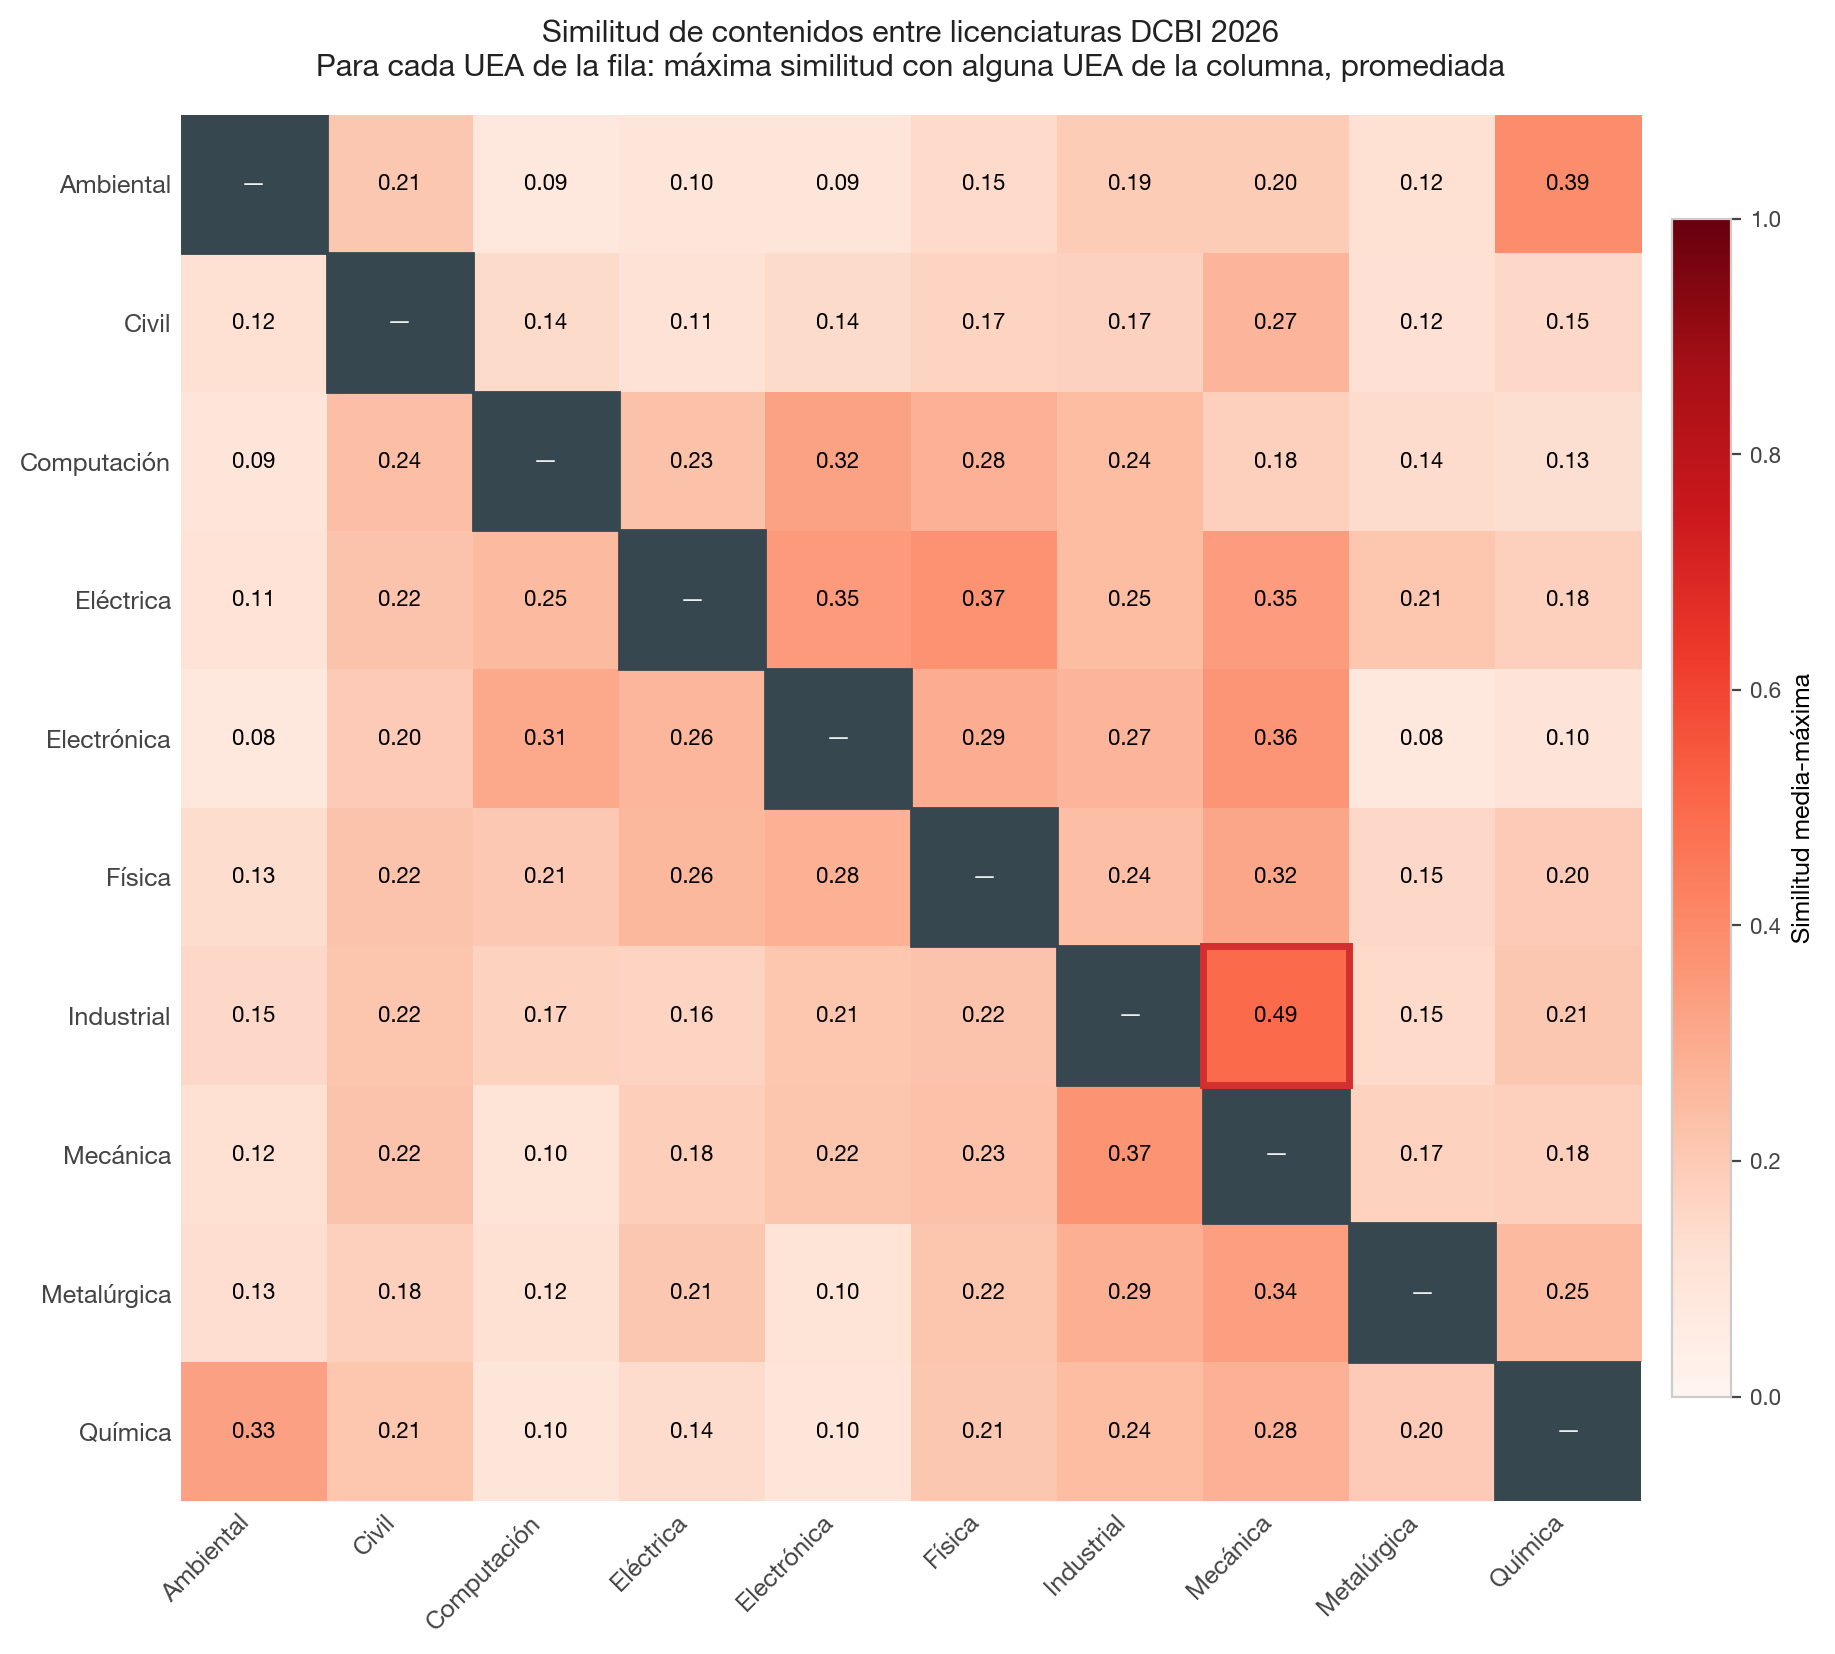
\includegraphics[width=0.82\textwidth]{Figuras/heatmap_licenciaturas.png}
  \caption{Similitud media-máxima $\simAB$ entre licenciaturas (ecuación~\eqref{eq:meanmax}).
    \emph{Cómo leer la figura.}
    La \emph{fila} indica el plan de origen $A$; la \emph{columna}, el plan de referencia $B$.
    La celda $(A,B)$ responde a: por cada UEA de $A$, ¿cuán similar es la UEA más parecida
    que existe en $B$? El valor reportado es el promedio de esa similitud máxima
    sobre todas las UEAs de $A$.
    La diagonal es 1 por definición (auto-similitud).
    \emph{Escala}: amarillo = baja similitud media-máxima; rojo oscuro = alta.
    \emph{Asimetría}: la celda $(A,B)$ puede diferir de $(B,A)$ cuando los planes difieren
    en tamaño o diversidad: un plan grande y diverso (como Mecánica, 108 UEAs) ofrece más
    oportunidades de encontrar contrapartes para las UEAs de cualquier otro plan,
    elevando la columna correspondiente.
    Una fila brillante indica que las UEAs de $A$ encuentran contrapartes similares
    en múltiples planes---señal de que $A$ comparte contenidos ampliamente.
    \emph{Patrones notables}: el par Ambiental--Química (celda brillante en ambas orientaciones)
    es el de mayor similitud bilateral; la fila de Física es uniformemente brillante,
    reflejando su alta conectividad transversal.}
  \label{fig:heatmap10}
\end{figure}

%%──────────────────────────────────────────────────────────────────────────
\subsection{Recuento de UEAs equivalentes: los 45 pares}
\label{sec:conteo}
%%──────────────────────────────────────────────────────────────────────────

La figura~\ref{fig:conteo_interplan} y la tabla~\ref{tab:matriz_interplan} cubren los $\binom{10}{2} = 45$ pares posibles de licenciaturas simultáneamente, mostrando cuántas UEAs comparte cada par a dos umbrales distintos.
A diferencia del mapa de calor anterior---que agrega la información en una métrica escalar por par---aquí se cuenta directamente el número de UEAs equivalentes, la magnitud más relevante para la revisión curricular.

\begin{figure}[H]
  \centering
  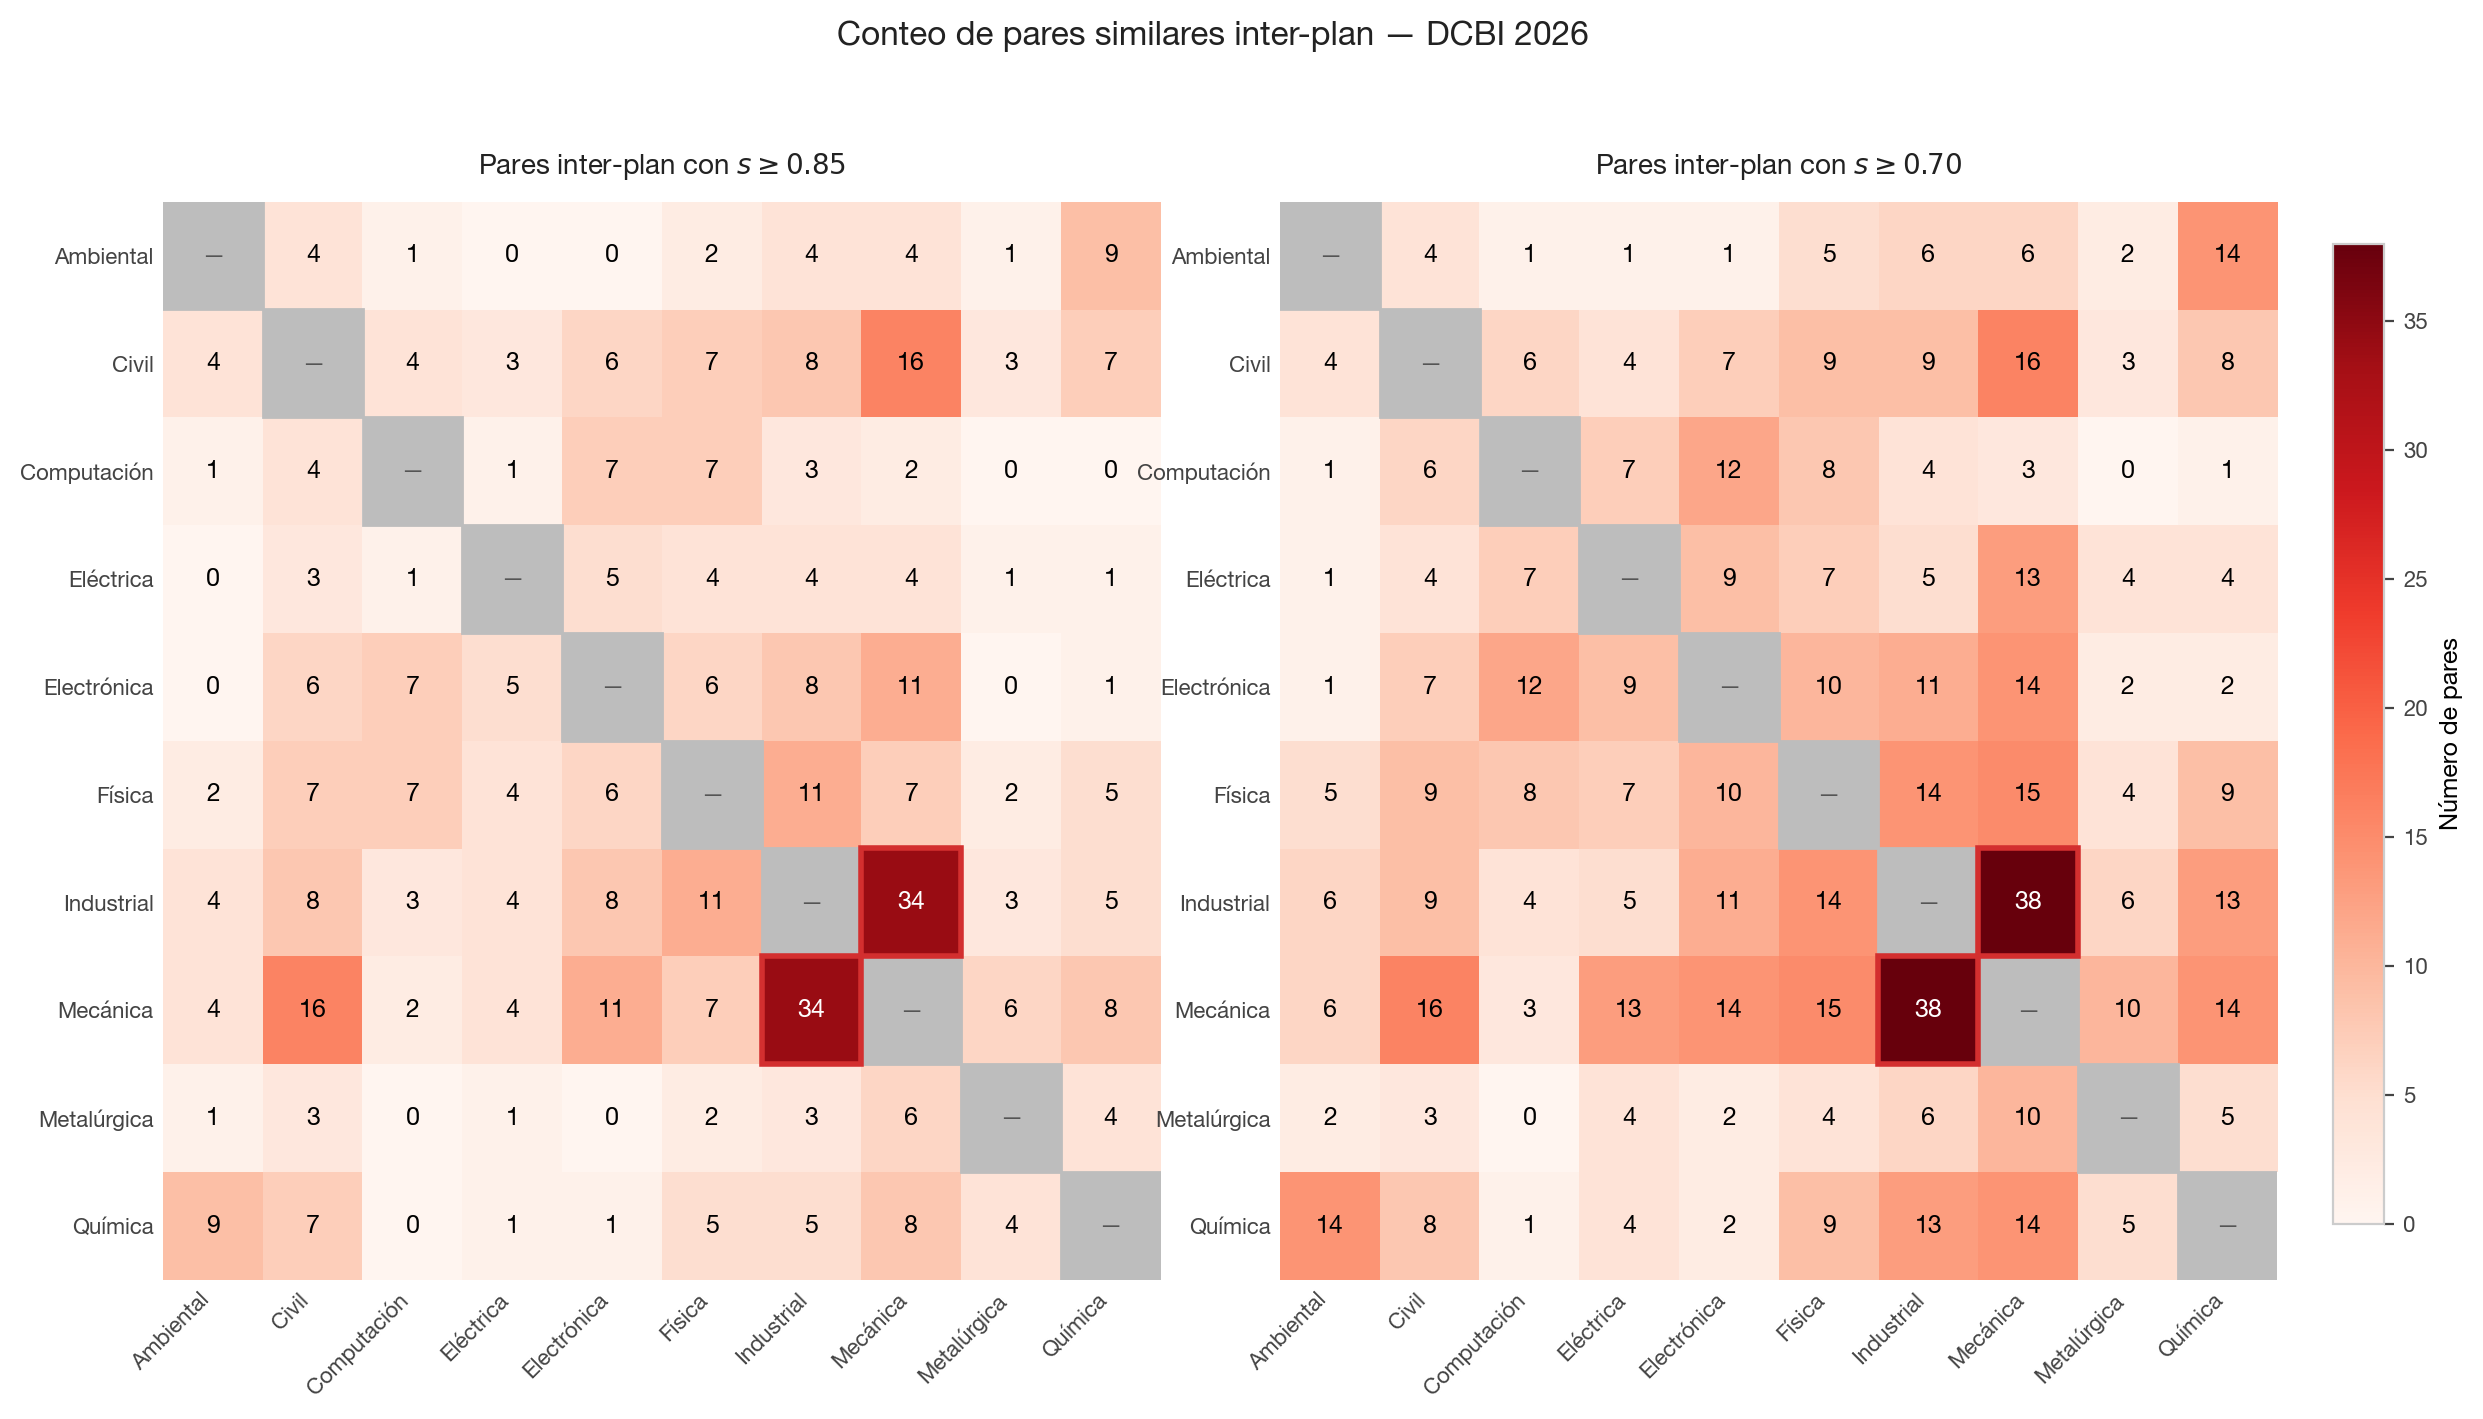
\includegraphics[width=\textwidth]{Figuras/heatmap_interplan_conteo.png}
  \caption{Número de UEAs equivalentes entre cada par de licenciaturas (los 45 pares).
    \emph{Cómo leer la figura.}
    Cada celda $(A,B)$ indica cuántas UEAs del par tienen $s(u_A, u_B) \geq$ umbral;
    la matriz es simétrica.
    Las celdas grises en la diagonal (intra-plan) no aplican.
    El guión ``---'' indica cero UEAs compartidas al umbral correspondiente.
    Ambos paneles comparten la misma escala de color (barra derecha, máximo = 38),
    por lo que los colores son directamente comparables entre paneles.
    \emph{Panel izquierdo}: umbral $s \geq 0.85$ (equivalencia muy alta).
    \emph{Panel derecho}: umbral $s \geq 0.70$ (equivalencia alta o mayor).
    Una celda que retiene su intensidad entre paneles indica que el traslape
    es mayoritariamente de equivalencia muy alta; una celda que palidece
    en el panel izquierdo tiene traslape real pero de calidad moderada-alta.
    \emph{Par dominante}: Industrial--Mecánica con 38 UEAs a $s \geq 0.70$
    y 34 a $s \geq 0.85$---la celda más oscura del corpus en ambos paneles.}
  \label{fig:conteo_interplan}
\end{figure}

\begin{table}[H]
\centering
\caption{Número de UEAs equivalentes a $s \geq 0.70$ entre cada par de licenciaturas
  (matriz híbrida TF-IDF + LLM, los 45 pares).
  Abreviaturas: Amb=Ambiental, Civ=Civil, Cmp=Computación, Elc=Eléctrica,
  Ele=Electrónica, Fis=Física, Ind=Industrial, Mec=Mecánica,
  Met=Metalúrgica, Qui=Química.}
\label{tab:matriz_interplan}
\footnotesize\setlength{\tabcolsep}{4pt}
\begin{tabular}{r *{10}{c}}
\toprule
 & \textbf{Amb} & \textbf{Civ} & \textbf{Cmp} & \textbf{Elc} & \textbf{Ele} & \textbf{Fis} & \textbf{Ind} & \textbf{Mec} & \textbf{Met} & \textbf{Qui} \\
\midrule
\textbf{Amb} & --- &  4 &  1 &  1 &  1 &  5 &  6 &  6 &  2 & 14 \\
\textbf{Civ} &  4  & --- &  6 &  4 &  7 &  9 &  9 & 16 &  3 &  8 \\
\textbf{Cmp} &  1  &  6  & --- &  7 & 12 &  8 &  4 &  3 &  0 &  1 \\
\textbf{Elc} &  1  &  4  &  7  & --- &  9 &  7 &  5 & 13 &  4 &  4 \\
\textbf{Ele} &  1  &  7  & 12  &  9  & --- & 10 & 11 & 14 &  2 &  2 \\
\textbf{Fis} &  5  &  9  &  8  &  7  & 10  & --- & 14 & 15 &  4 &  9 \\
\textbf{Ind} &  6  &  9  &  4  &  5  & 11  & 14  & --- & 38 &  6 & 13 \\
\textbf{Mec} &  6  & 16  &  3  & 13  & 14  & 15  & 38  & --- & 10 & 14 \\
\textbf{Met} &  2  &  3  &  0  &  4  &  2  &  4  &  6  & 10  & --- &  5 \\
\textbf{Qui} & 14  &  8  &  1  &  4  &  2  &  9  & 13  & 14  &  5  & --- \\
\bottomrule
\end{tabular}
\end{table}

%%──────────────────────────────────────────────────────────────────────────
\subsection{Red de traslape}
\label{sec:grafo}
%%──────────────────────────────────────────────────────────────────────────

\begin{figure}[H]
  \centering
  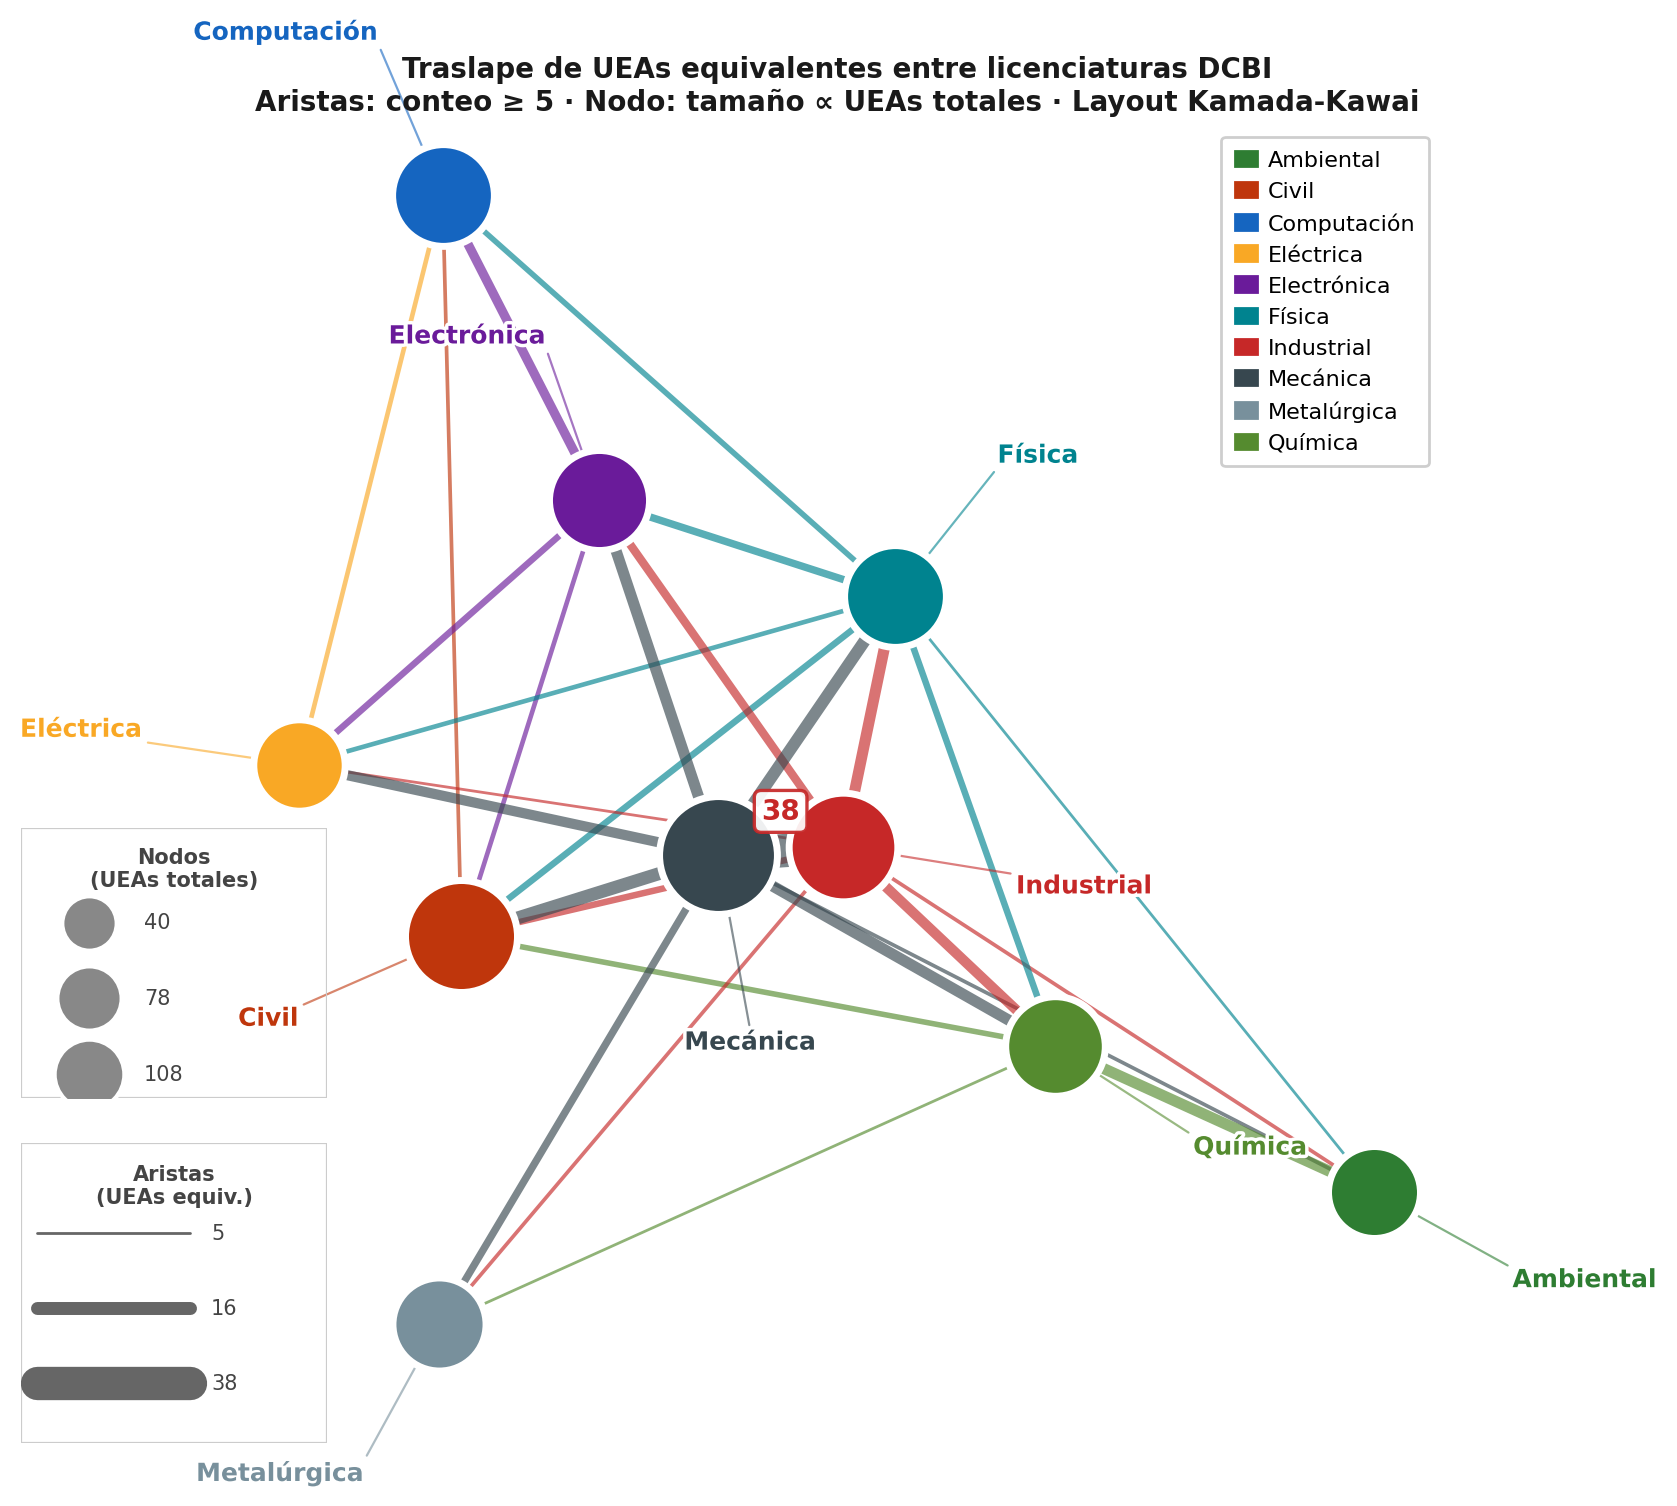
\includegraphics[width=0.90\textwidth]{Figuras/grafo_licenciaturas_variante_B.png}
  \caption{Red de traslape entre licenciaturas --- pares con $\geq 5$ UEAs equivalentes
    a $s \geq 0.70$ (29 de los 45 pares posibles; los 16 pares con $< 5$ UEAs no tienen arista).
    \emph{Cómo leer la figura.}
    Cada \emph{nodo} representa una licenciatura; su \emph{área} es proporcional
    al número de UEAs en el corpus (Mecánica~=~108 UEAs, el más grande;
    Eléctrica~=~39, el más pequeño; ver escala en la leyenda inferior izquierda).
    El \emph{color} del nodo identifica la licenciatura (ver leyenda derecha).
    Cada \emph{arista} conecta dos licenciaturas con $\geq 5$ UEAs equivalentes;
    su \emph{grosor} es proporcional al conteo (escala de aristas en la leyenda:
    5, 16 y 38 UEAs).
    El número \textbf{38} anotado sobre la arista entre Industrial y Mecánica
    indica el conteo máximo del corpus, seis veces mayor que el segundo par más alto.
    La \emph{posición espacial} (layout Kamada-Kawai, distancia $\propto 1/\text{conteo}$)
    agrupa automáticamente las licenciaturas con mayor traslape mutuo:
    el bloque Mecánica--Industrial--Física--Electrónica--Civil converge en el centro;
    Ambiental y Química quedan juntas en la periferia por su bloque disciplinar compartido.
    \emph{Ausencia notable}: Computación y Metalúrgica no están conectadas ---el único
    par de los 45 con cero UEAs equivalentes a $s \geq 0.70$.}
  \label{fig:grafoLic}
\end{figure}

%%──────────────────────────────────────────────────────────────────────────
\subsection{UEAs con mayor presencia transversal}
\label{sec:transversal}
%%──────────────────────────────────────────────────────────────────────────

La tabla~\ref{tab:transversal} identifica qué UEAs específicas son responsables del traslape inter-plan, agrupando las que aparecen en tres o más licenciaturas con $s \geq 0.70$.
La columna $n$ indica el número de licenciaturas; $s_\text{máx}$ es la similitud máxima observada en cualquier par de esa UEA.
Abreviaturas: \textsf{Amb}=Ambiental, \textsf{Civ}=Civil, \textsf{Cmp}=Computación, \textsf{Elc}=Eléctrica, \textsf{Ele}=Electrónica, \textsf{Fis}=Física, \textsf{Ind}=Industrial, \textsf{Mec}=Mecánica, \textsf{Met}=Metalúrgica, \textsf{Qui}=Química.

\begin{table}[H]
\centering
\caption{UEAs presentes en tres o más licenciaturas con $s \geq 0.70$ (matriz híbrida).
  ${}^{*}$ Familia de UEAs con el mismo contenido pero distintas claves en cada plan;
  no excluida como TG por el algoritmo de exclusión basado en clave.
  ${}^{\dagger}$ Invisible a TF-IDF ($s_{\mathrm{TF}} \approx 0.21$--$0.25$);
  detectada como equivalente exclusivamente por el LLM.}
\label{tab:transversal}
\footnotesize\setlength{\tabcolsep}{5pt}
\begin{tabular}{p{5.8cm} c c p{5.5cm}}
\toprule
\textbf{UEA} & \bm{$n$} & \bm{$s_\text{máx}$} & \textbf{Licenciaturas} \\
\midrule
\multicolumn{4}{l}{\textit{Presentes en 6 o más planes}} \\
\addlinespace[2pt]
Ecuaciones Diferenciales (Ord.)${}^{*}$ & 9 & 1.000 & Amb, Civ, Elc, Ele, Fis, Ind, Mec, Met, Qui \\
Liderazgo y Emprendimiento${}^{\dagger}$  & 9 & 0.950 & Amb, Civ, Cmp, Elc, Ele, Fis, Ind, Mec, Met \\
Educación Ambiental y Cambio Climático  & 6 & 1.000 & Civ, Elc, Ele, Fis, Mec, Qui \\
Taller de Comunicación Técnica y Prof.  & 6 & 0.990 & Civ, Cmp, Ele, Fis, Ind, Mec \\
\addlinespace[4pt]
\multicolumn{4}{l}{\textit{Presentes en 5 planes}} \\
\addlinespace[2pt]
Cálculo Integral               & 5 & 1.000 & Civ, Cmp, Ele, Fis, Mec \\
Gestión y Seguimiento de Proyectos & 5 & 1.000 & Cmp, Elc, Ele, Fis, Ind \\
Estructura y Prop.\@ de los Materiales & 5 & 0.980 & Amb, Fis, Ind, Mec, Qui \\
Métodos Numéricos en Ingeniería  & 5 & 0.980 & Civ, Elc, Mec, Met, Qui \\
Probabilidad y Estadística Descr. & 5 & 0.980 & Civ, Ele, Fis, Ind, Mec \\
Programación Aplic.\@ a la Ingeniería & 5 & 0.980 & Civ, Fis, Ind, Mec, Met \\
\addlinespace[4pt]
\multicolumn{4}{l}{\textit{Presentes en 4 planes}} \\
\addlinespace[2pt]
Herramientas Digitales en Ingeniería & 4 & 1.000 & Civ, Fis, Ind, Qui \\
Lab.\@ de Estr.\@ y Prop.\@ de Materiales & 4 & 0.980 & Fis, Ind, Mec, Qui \\
Energía Solar Fotovoltaica       & 4 & 0.980 & Elc, Fis, Ind, Mec \\
Diseño Digital                   & 4 & 0.980 & Cmp, Elc, Ele, Mec \\
\addlinespace[4pt]
\multicolumn{4}{l}{\textit{Presentes en 3 planes con $s = 1.00$}} \\
\addlinespace[2pt]
Análisis de Ciclo de Vida        & 3 & 1.000 & Amb, Civ, Qui \\
Ingeniería Económica             & 3 & 1.000 & Ind, Mec, Qui \\
Seguridad e Higiene Industrial   & 3 & 1.000 & Ind, Mec, Qui \\
Análisis de Costos para Toma de Dec. & 3 & 1.000 & Elc, Ind, Mec \\
Evaluación de Proyectos en Ing.  & 3 & 1.000 & Ele, Ind, Mec \\
Dibujo Asistido por Computadora  & 3 & 1.000 & Civ, Ele, Elc \\
\bottomrule
\end{tabular}
\end{table}

%%──────────────────────────────────────────────────────────────────────────
\subsection{Pares individuales de mayor similitud}
\label{sec:top_inter}
%%──────────────────────────────────────────────────────────────────────────

La tabla~\ref{tab:inter} lista los veinte pares de UEAs individuales con mayor puntuación en la matriz híbrida.
$s = 1.00$ indica equivalencia textual; $s \geq 0.92$ indica equivalencia semántica muy alta.

\begin{table}[H]
\centering
\caption{Veinte pares inter-plan de mayor similitud (matriz híbrida TF-IDF + LLM).
  $s = 1.00$: programas con contenido textualmente idéntico.
  $s \geq 0.92$: equivalencia semántica muy alta confirmada por el LLM.}
\label{tab:inter}
\small\setlength{\tabcolsep}{4pt}
\begin{tabular}{clll}
\toprule
\textbf{Sim.} & \textbf{Nombre de la UEA} & \textbf{Lic.\@ A} & \textbf{Lic.\@ B} \\
\midrule
1.000 & Análisis de Ciclo de Vida           & Ambiental   & Química \\
1.000 & Manejo y Tratam.\@ de Residuos Ind. & Ambiental   & Química \\
1.000 & Educación Ambiental y Cambio Clim.  & Civil       & Química \\
1.000 & Ecuaciones Diferenciales            & Electrónica & Física  \\
0.980 & Análisis de Ciclo de Vida           & Ambiental   & Química \\
0.980 & Procesos Biológicos en Ing.\@ Amb.  & Ambiental   & Química \\
0.980 & Educación Ambiental y Cambio Clim.  & Electrónica & Química \\
0.980 & Lab.\@ Estructura y Prop.\@ Mat.    & Física      & Química \\
0.950 & Microbiología Aplicada              & Ambiental   & Química \\
0.950 & Estructura y Prop.\@ de Materiales  & Ambiental   & Química \\
0.950 & Legislación y Gestión Ambiental     & Ambiental   & Química \\
0.950 & Mecánica de Fluidos                 & Ambiental   & Química \\
0.950 & Ecuaciones Diferenciales Ordinarias & Civil       & Mecánica \\
0.950 & Análisis de Ciclo de Vida           & Civil       & Química \\
0.950 & Álgebra Lineal                      & Computación & Física  \\
0.950 & Ética, Respons.\@ Social y Sost.    & Computación & Física  \\
0.950 & Estadística                         & Computación & Física  \\
0.950 & Liderazgo y Emprendimiento          & Computación & Física  \\
0.950 & Educación Ambiental y Cambio Clim.  & Eléctrica   & Química \\
0.920 & Ing.\@ de los Materiales            & Industrial  & Metalúrgica \\
\bottomrule
\end{tabular}
\end{table}

Los veinte pares de la tabla~\ref{tab:inter} concentran cuatro fenómenos distintos.
El bloque Ambiental--Química domina la parte superior con ocho pares (y una docena adicional con $s \geq 0.70$ no mostrados).
``Educación Ambiental y Cambio Climático'' aparece en tres instancias en la tabla y está presente en al menos seis planes (tabla~\ref{tab:transversal}).
La fila Computación--Física agrupa cuatro UEAs de formación amplia (Álgebra Lineal, Ética, Estadística, Liderazgo) con $s = 0.95$.
El par Civil--Mecánica en Ecuaciones Diferenciales Ordinarias introduce el núcleo matemático transversal documentado en la tabla~\ref{tab:transversal}.

%% ════════════════════════════════════════════════════════════════════════════
\section{Análisis intra-plan}
\label{sec:intra}
%% ════════════════════════════════════════════════════════════════════════════

Esta sección analiza la similitud entre UEAs \textit{dentro de un mismo plan}.
Alta similitud intra-plan puede deberse a causas legítimas---una pareja taller/teoría del mismo nombre base es un par esperado---o a causas problemáticas: UEAs de distinto nivel con contenido no diferenciado, o duplicaciones documentales.

%%──────────────────────────────────────────────────────────────────────────
\subsection{Pares y casos más relevantes}
%%──────────────────────────────────────────────────────────────────────────

\begin{table}[H]
\centering
\caption{Quince pares intra-plan de mayor similitud (matriz híbrida TF-IDF + LLM).
  $\dagger$~pareja taller/teoría confirmada como legítima por el LLM.
  Sin marca: par que requiere revisión curricular.}
\label{tab:intra}
\small\setlength{\tabcolsep}{4pt}
\begin{tabular}{clcl}
\toprule
\textbf{Sim.} & \textbf{UEA A} & \textbf{Lic.} & \textbf{UEA B} \\
\midrule
0.990 & Análisis de Ciclo de Vida          & Química    & Análisis de Ciclo de Vida (dup.) \\
0.950 & Aplic.\@ Exp.\@ Ing.\@ Física I   & Física     & Aplic.\@ Exp.\@ Ing.\@ Física II \\
0.880 & Taller Inv.\@ en Ing.\@ Civil I    & Civil      & Taller Inv.\@ en Ing.\@ Civil II \\
0.850$^\dagger$ & Lab.\@ de Metrología para Manufactura & Industrial & Metrología para Manufactura \\
0.850$^\dagger$ & Lab.\@ de Eficiencia Operativa    & Industrial & Medición del Trabajo p.\@ Eficiencia \\
0.850$^\dagger$ & Taller de Tecn.\@ de Conformado   & Industrial & Tecn.\@ de Conformado y Ensamble \\
0.850$^\dagger$ & Lab.\@ de Mecanismos              & Mecánica   & Mecanismos \\
0.850$^\dagger$ & Proy.\@ Mecánico de Montajes       & Mecánica   & Taller Proy.\@ Mecánico de Montajes \\
0.850$^\dagger$ & Lab.\@ de Eficiencia Operativa    & Mecánica   & Medición del Trabajo p.\@ Eficiencia \\
0.820 & Elementos de Acero                 & Civil      & Diseño de Estructuras de Acero \\
0.780$^\dagger$ & Estructura y Prop.\@ de Materiales & Industrial & Lab.\@ de Estr.\@ y Prop.\@ de Mat. \\
0.780$^\dagger$ & Estructura y Prop.\@ de Materiales & Mecánica   & Lab.\@ de Estr.\@ y Prop.\@ de Mat. \\
0.780$^\dagger$ & Taller de Tecn.\@ de Conformado   & Mecánica   & Tecn.\@ de Conformado y Ensamble \\
0.780$^\dagger$ & Calefacción, Vent.\@ y Aire Acond. & Mecánica  & Taller de CVAA \\
0.780$^\dagger$ & Tratamientos Térmicos de Mat.      & Metalúrgica & Lab.\@ de Tratamientos Térmicos \\
\bottomrule
\end{tabular}
\end{table}

Los tres primeros pares de la tabla~\ref{tab:intra} son casos problemáticos; los doce restantes son parejas taller/teoría confirmadas como legítimas por el LLM.

\textbf{Caso 1: Química --- duplicado de ``Análisis de Ciclo de Vida'' ($s = 0.990$).}
El corpus contiene dos documentos con el mismo título y contenido.
Debe determinarse cuál es el programa vigente y retirarse el duplicado del repositorio.

\textbf{Caso 2: Física --- ``Aplic.\@ Exp.\@ Ing.\@ Física I'' y ``II'' ($s = 0.950$).}
Dos UEAs consecutivas de laboratorio evaluadas como \textit{idéntico} por el LLM.
O bien los campos de Objetivo General y Contenido Sintético no han sido diferenciados entre niveles, o bien se trata de una duplicación documental.

\textbf{Caso 3: Civil --- Taller de Investigación I vs.\  II ($s = 0.880$).}
Dos instancias del mismo tipo de actividad en trimestres consecutivos sin diferenciación de programa.
Civil concentra 61 pares intra-plan a $s \geq 0.40$ (el mayor del corpus): el LLM detectó que las áreas de estructuras, hidráulica, geotecnia y materiales comparten objetivos convergentes redactados independientemente por departamentos distintos.

\textbf{Caso adicional --- Industrial: duplicado de ``Herramientas Digitales en Ingeniería'' (clave 1100202).}
Dos documentos con la misma clave y contenido en el corpus de Industrial.
No aparece en la tabla~\ref{tab:intra} porque la detección automática excluye pares con clave idéntica; fue identificado mediante el mapa de calor intra-plan.

%%──────────────────────────────────────────────────────────────────────────
\subsection{Mapas de calor intra-plan}
%%──────────────────────────────────────────────────────────────────────────

Las figuras~\ref{fig:intra_civil}--\ref{fig:intra_elecn} son los mapas de calor intra-plan de las diez licenciaturas, ordenados de mayor a menor densidad de traslape.

\paragraph{Cómo leer los mapas.}
Filas y columnas corresponden a las UEAs del plan, reordenadas por agrupamiento jerárquico de Ward: las UEAs de contenido similar quedan contiguas.
\emph{Diagonal}: siempre 1 (auto-similitud); una franja roja continua en la diagonal sin bloques off-diagonal indica plan bien diferenciado.
\emph{Bloque compacto cerca de la diagonal}: grupo de UEAs temáticamente afines (por ejemplo, un área disciplinar con varias materias relacionadas o una secuencia taller/teoría).
\emph{Celda brillante aislada fuera de la diagonal}: par puntual de alta similitud---puede ser una pareja taller/teoría legítima o un duplicado problemático.
\emph{Escala}: amarillo claro = baja similitud; rojo intenso = alta.
Los planes con más de 55 UEAs se presentan sin etiquetas de eje (ilegibles a textwidth); la versión interactiva identifica cada UEA al pasar el cursor.

%%── Civil ────────────────────────────────────────────────────────────────────

\paragraph{Civil (88 UEAs, 61 pares con $s \geq 0.40$).}
La licenciatura con mayor densidad de traslape intra-plan del corpus.
El mapa muestra múltiples bloques de color intenso distribuidos en la diagonal, correspondientes a grupos de estructuras, hidráulica y materiales con objetivos convergentes.
La celda más brillante corresponde a Taller de Investigación I vs.\ II ($s = 0.880$, Caso~3); Elementos de Acero/Diseño de Estructuras de Acero ($s = 0.820$) es el par teoría/aplicación más significativo.

\begin{figure}[H]
  \centering
  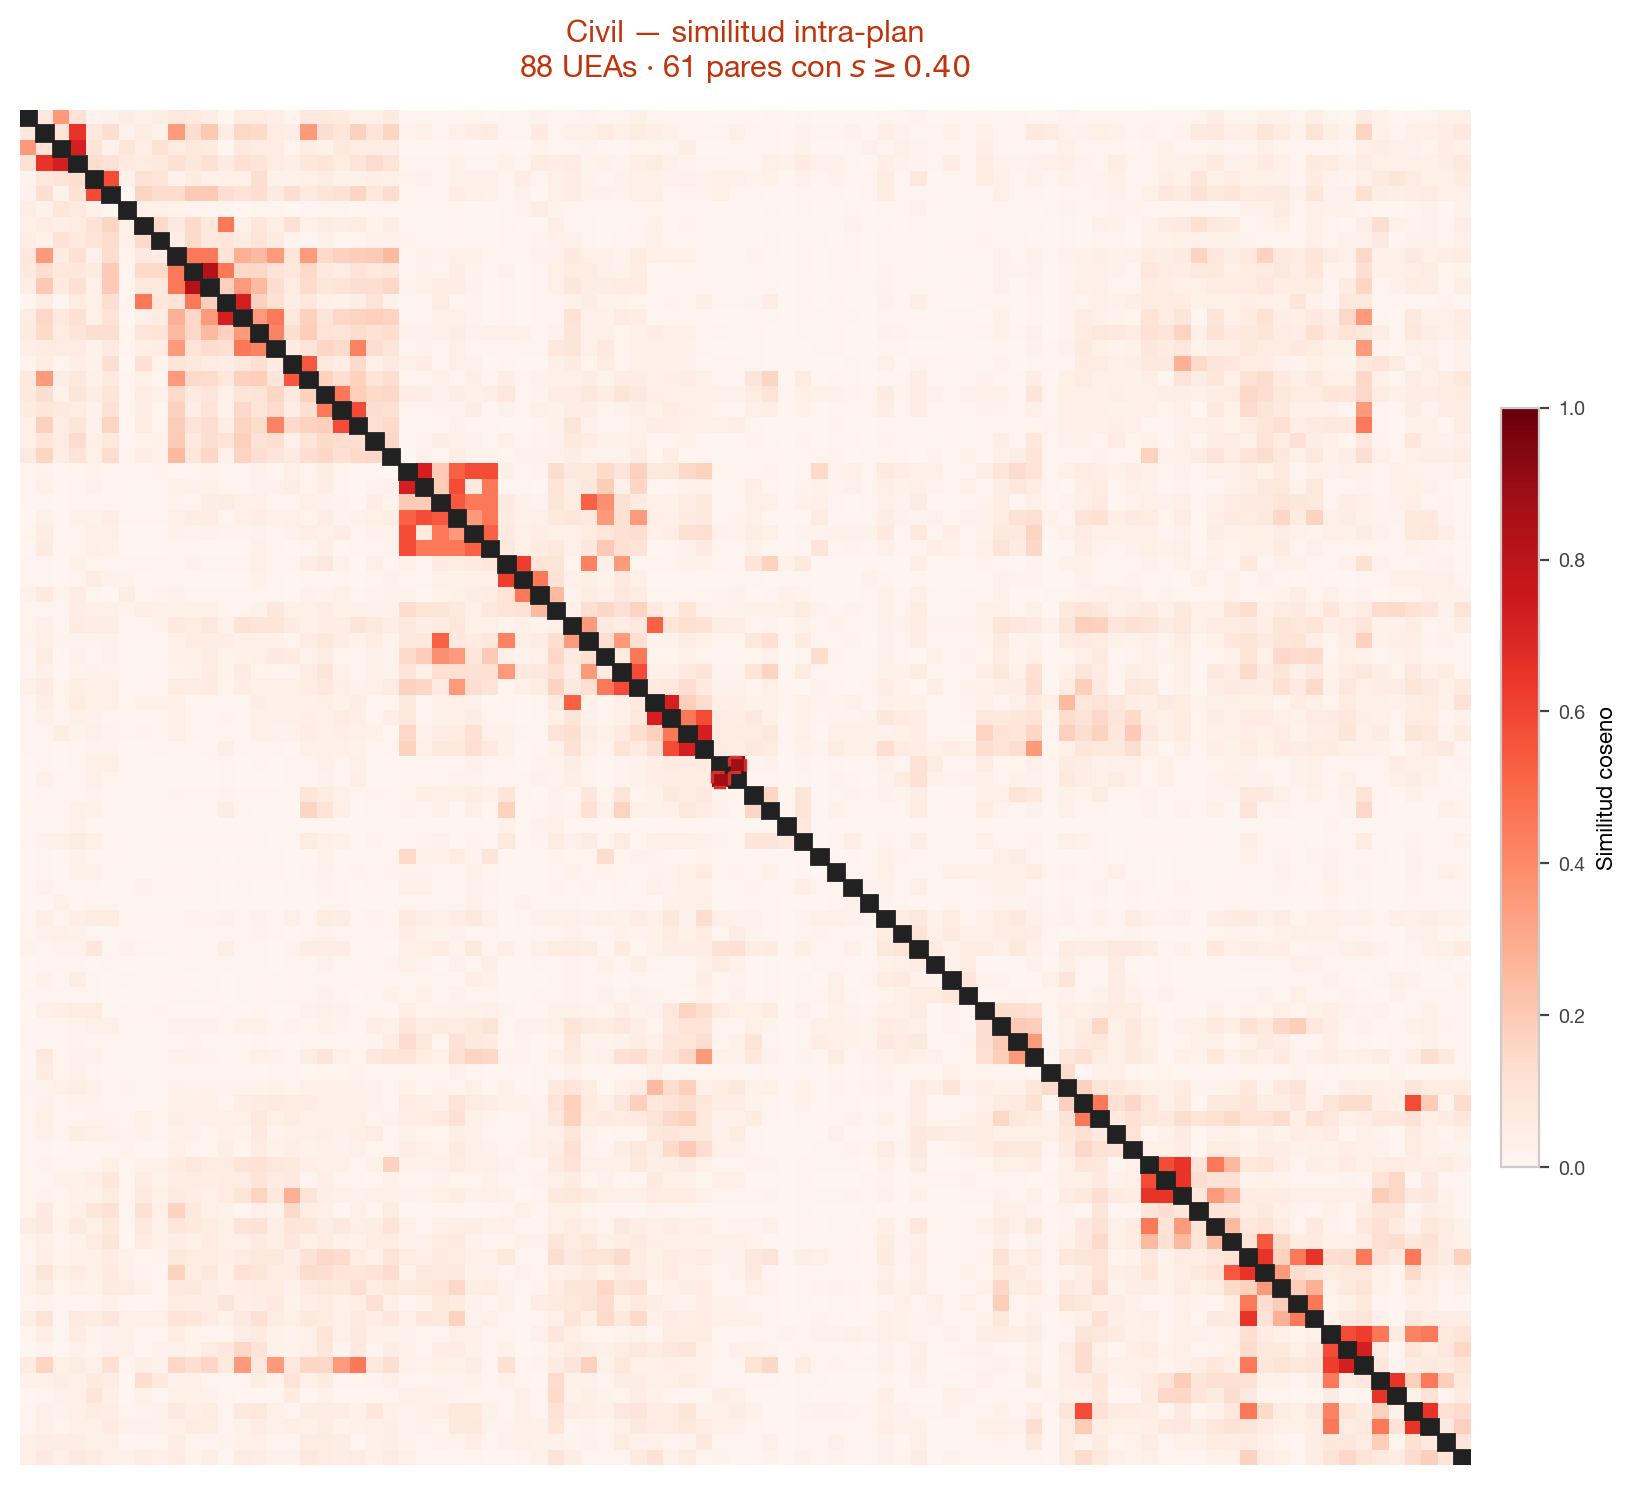
\includegraphics[width=\textwidth]{Figuras/intraplan_Civil.png}
  \caption{Similitud intra-plan --- Civil (88 UEAs, 61 pares con $s \geq 0.40$).
    La alta densidad de bloques en la diagonal refleja objetivos convergentes
    en las áreas de estructuras, hidráulica, geotecnia y materiales---redactados
    independientemente por departamentos distintos y detectados como equivalentes
    por el LLM (TF-IDF reportaba solo 8 pares).
    La celda más brillante: Taller Inv.\ Civil I vs.\ II ($s = 0.880$, Caso~3).
    Ver \texttt{intraplan\_Civil.html} para identificar UEAs individuales.}
  \label{fig:intra_civil}
\end{figure}

%%── Metalúrgica ──────────────────────────────────────────────────────────────

\paragraph{Metalúrgica (42 UEAs, 29 pares con $s \geq 0.40$).}
El mayor incremento relativo del corpus: de 3 pares (TF-IDF) a 29 (LLM).
El vocabulario técnico especializado de Metalúrgica es heterogéneo entre versiones del mismo programa, lo que impedía la detección léxica; el LLM reconoció la equivalencia semántica.
Los 29 pares son en su totalidad parejas taller/teoría o áreas afines; no se identifican duplicados ni pares problemáticos.
El par más alto es Lab.\@ de Tratamientos Térmicos/Tratamientos Térmicos de los Materiales ($s = 0.780$).

\begin{figure}[H]
  \centering
  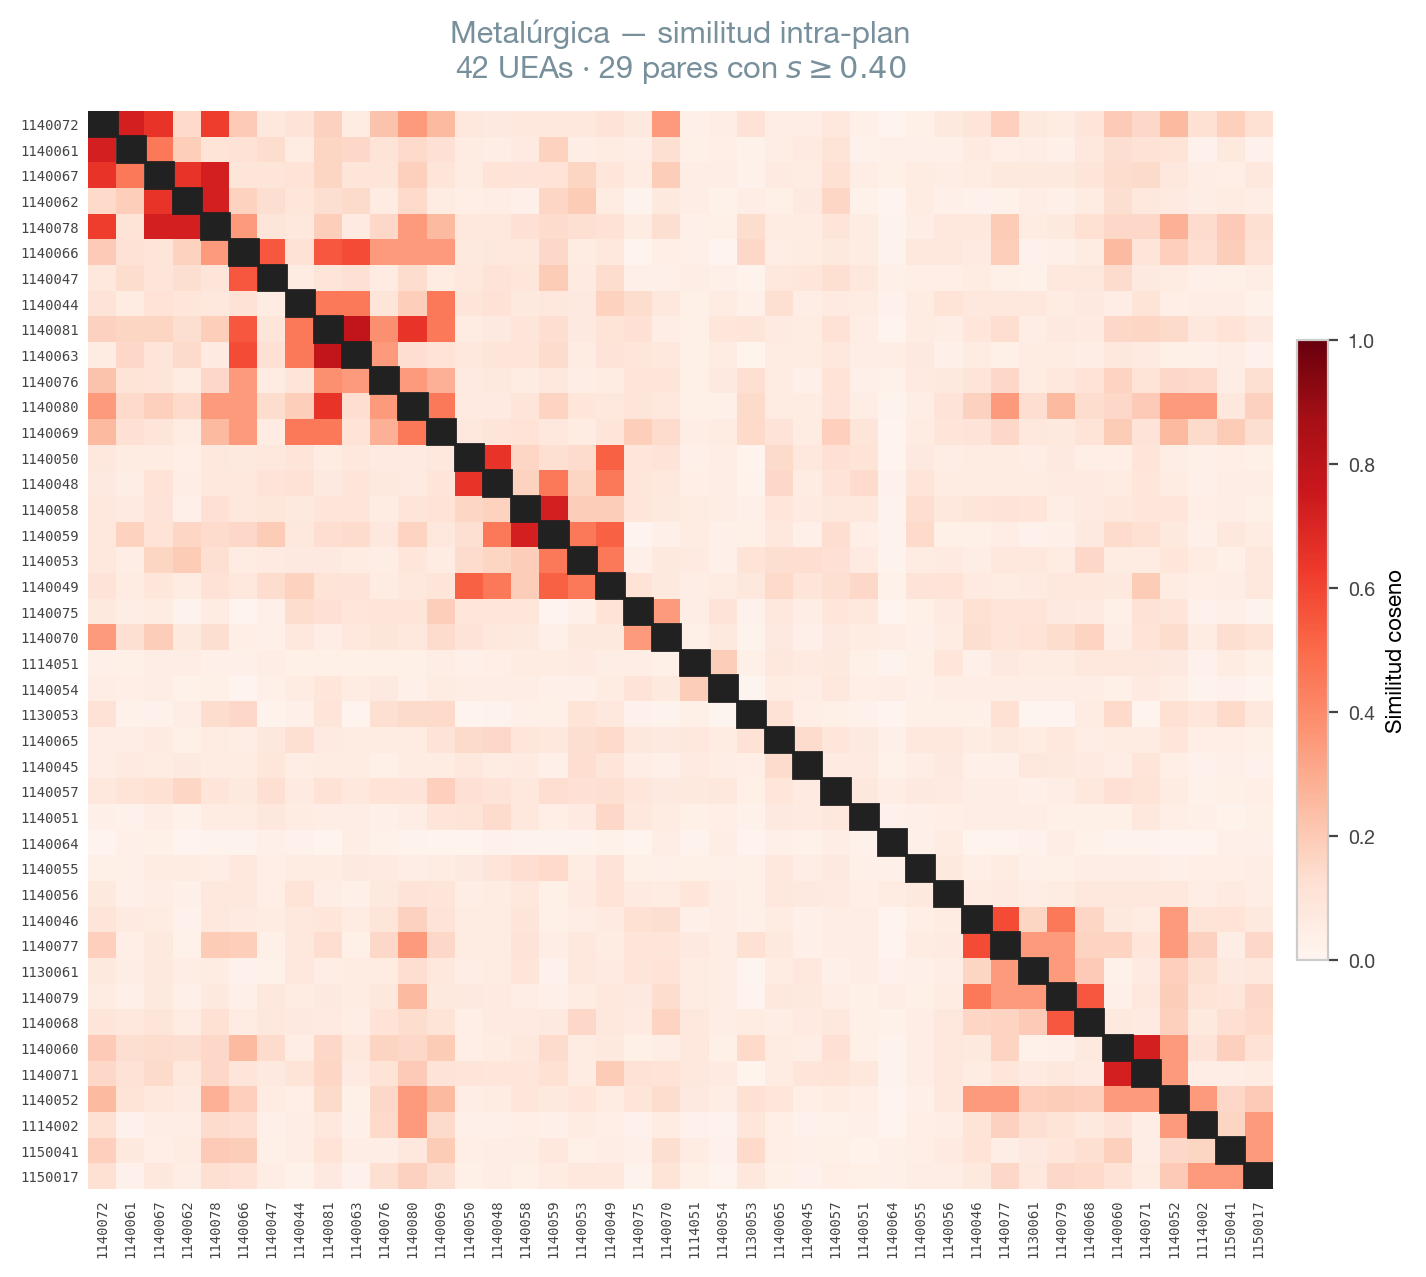
\includegraphics[width=0.76\textwidth]{Figuras/intraplan_Metalurgica.png}
  \caption{Similitud intra-plan --- Metalúrgica (42 UEAs, 29 pares con $s \geq 0.40$).
    El patrón de bloques en la diagonal corresponde a parejas taller/teoría
    del área de materiales y procesos (tratamientos térmicos, metalografía, soldadura).
    El salto de 3 a 29 pares respecto a TF-IDF refleja vocabulario técnico
    heterogéneo entre versiones del mismo programa, no duplicados.}
  \label{fig:intra_met}
\end{figure}

%%── Computación ─────────────────────────────────────────────────────────────

\paragraph{Computación (60 UEAs, 33 pares con $s \geq 0.40$).}
El LLM redujo los pares de 57 (TF-IDF) a 33, descartando 24 artefactos léxicos del vocabulario genérico de software.
Se distinguen dos bloques de traslape genuino: el área de \textit{bases de datos} (Relacional, No Relacional, Distribuida) y el área de \textit{redes} (Redes de Computadoras, Administración, Seguridad, Automatización).
El par Programación Orientada a Objetos I vs.\ II permanece como el par no-taller más preocupante.

\begin{figure}[H]
  \centering
  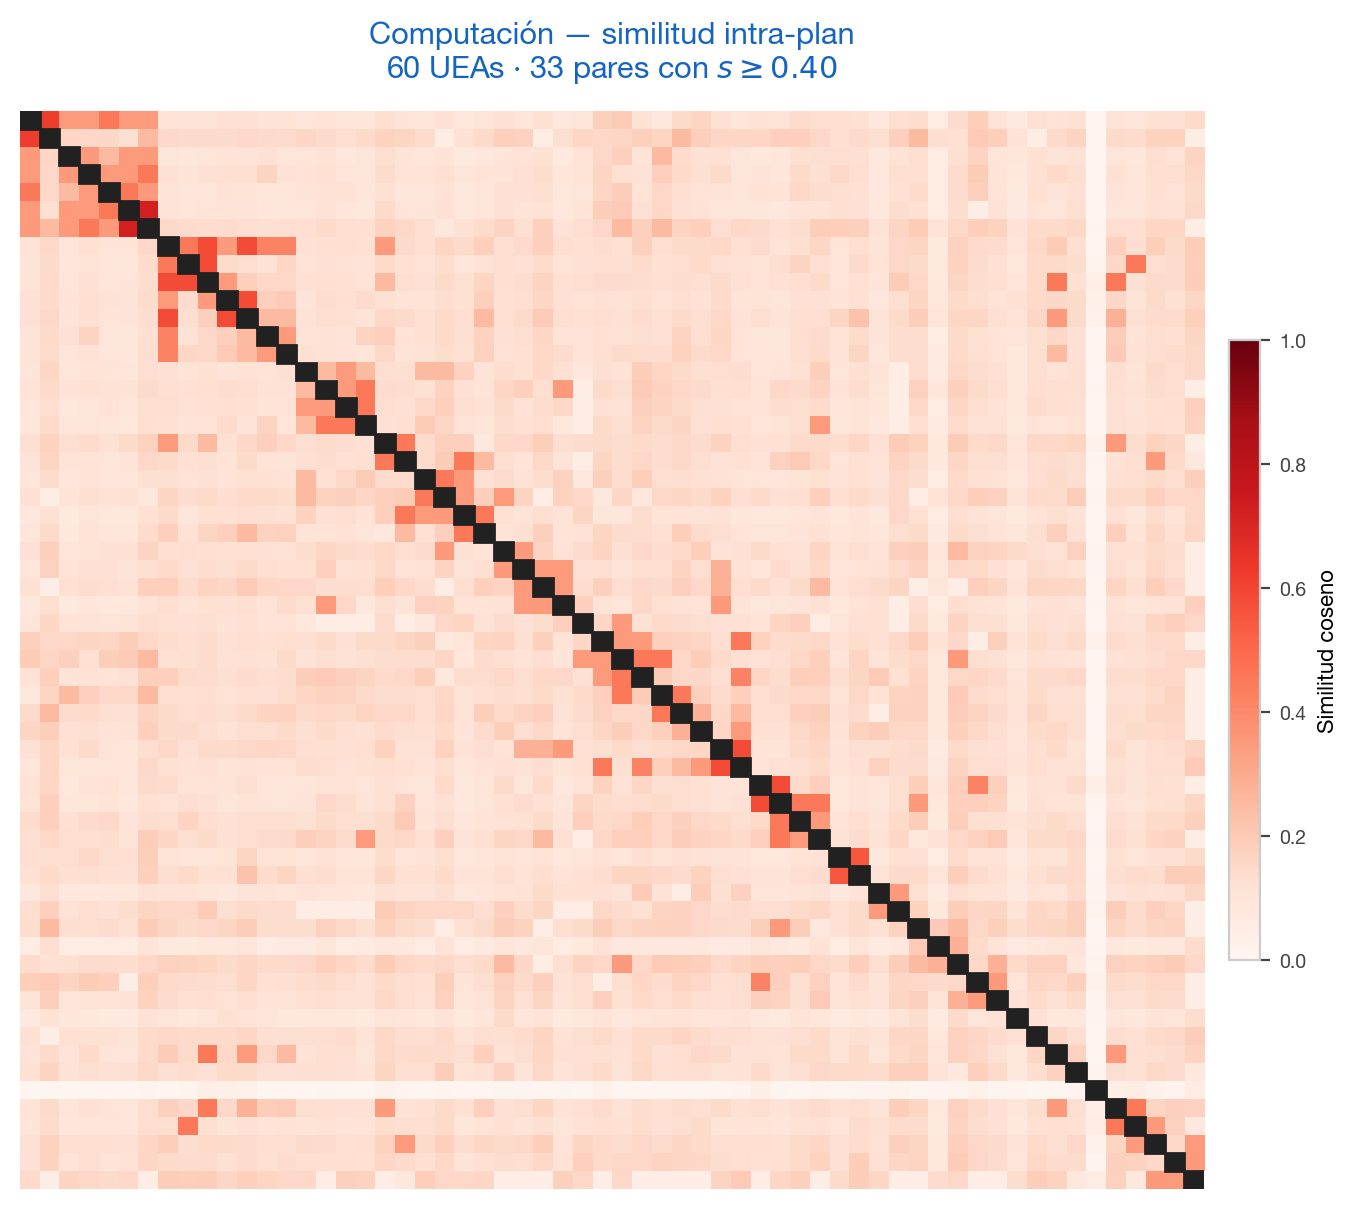
\includegraphics[width=\textwidth]{Figuras/intraplan_Computacion.png}
  \caption{Similitud intra-plan --- Computación (60 UEAs, 33 pares con $s \geq 0.40$).
    Se distinguen dos bloques de traslape genuino: el área de bases de datos
    (tres UEAs con objetivos solapados) y el área de redes (cuatro UEAs afines).
    El punto brillante aislado en la esquina corresponde a POO I vs.\ II.
    TF-IDF reportaba 57 pares; el LLM descartó 24 como falsos positivos
    atribuibles a vocabulario genérico de desarrollo de software.
    Ver \texttt{intraplan\_Computacion.html} para identificar UEAs individuales.}
  \label{fig:intra_comp}
\end{figure}

%%── Mecánica ─────────────────────────────────────────────────────────────

\paragraph{Mecánica (108 UEAs, 25 pares con $s \geq 0.40$).}
El plan más extenso del corpus.
La mayor parte del mapa es de color frío, indicando que los 108 contenidos están bien diferenciados para un plan de esta magnitud.
Los 25 pares son todos parejas taller/laboratorio esperadas: Lab.\@ de Mecanismos/Mecanismos ($s = 0.85$), Lab.\@ de Eficiencia Operativa/Medición del Trabajo ($s = 0.85$), Lab.\@ Estructura y Prop./Estructura y Prop.\@ de Mat.\@ ($s = 0.78$), Taller de CVAA/CVAA ($s = 0.78$).

\begin{figure}[H]
  \centering
  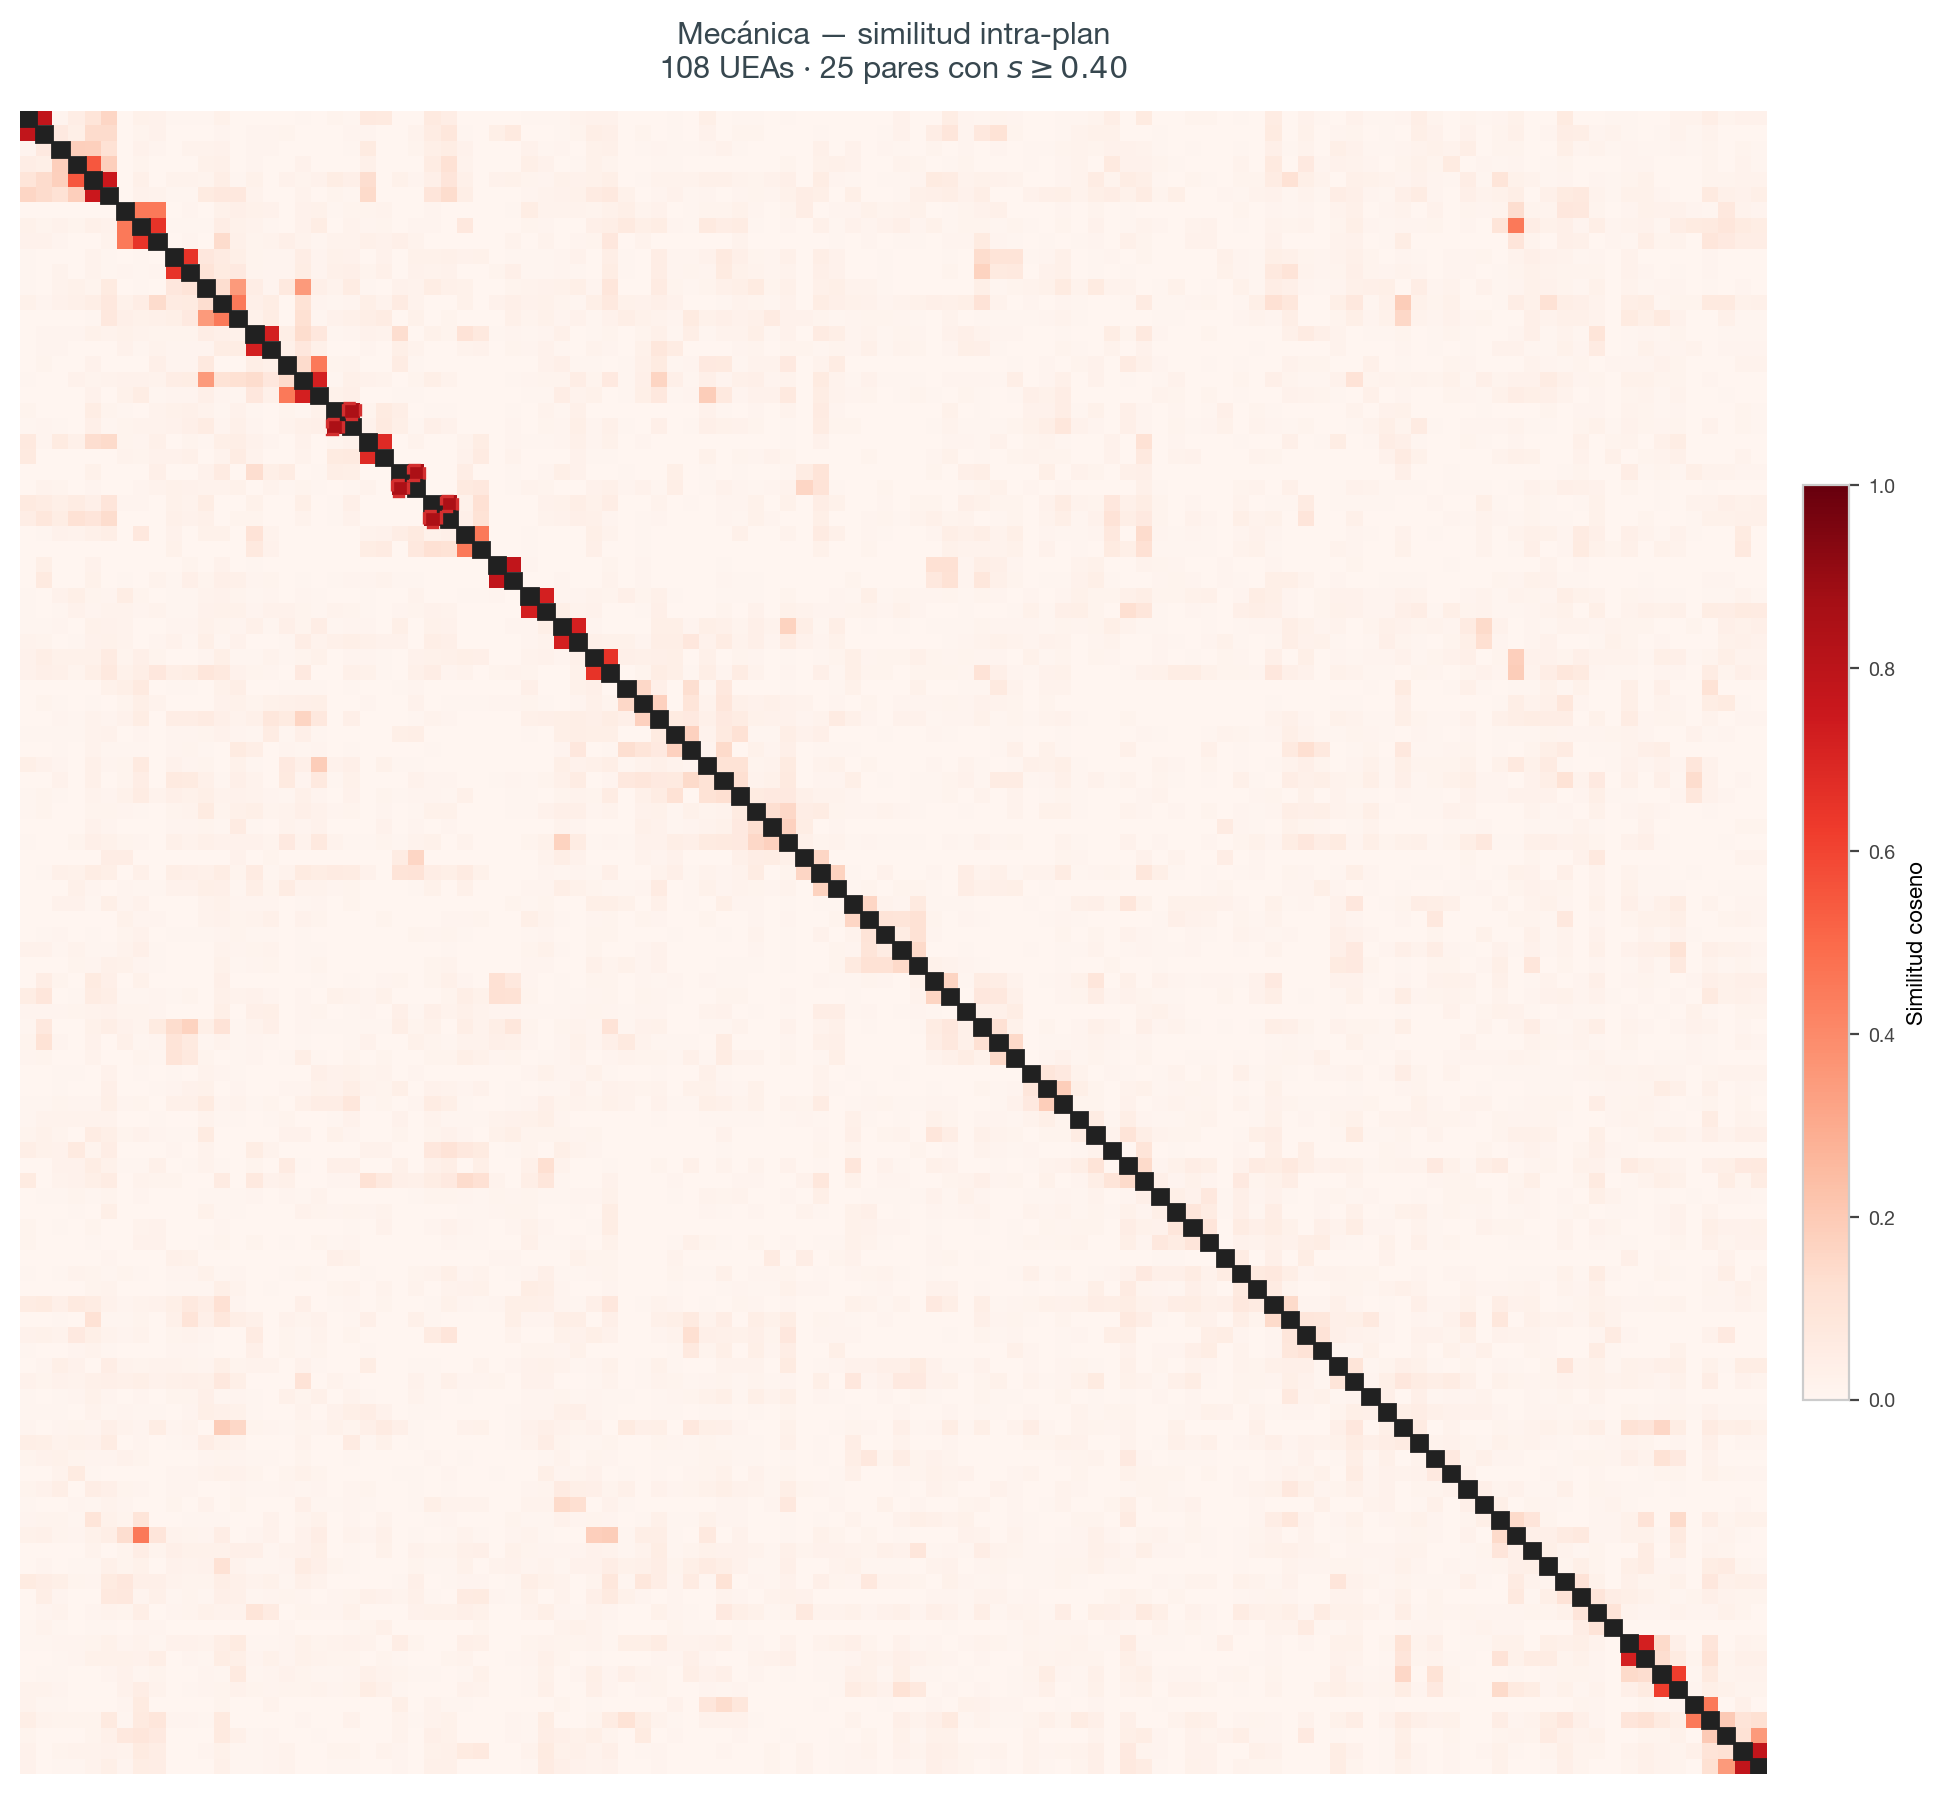
\includegraphics[width=\textwidth]{Figuras/intraplan_Mecanica.png}
  \caption{Similitud intra-plan --- Mecánica (108 UEAs, 25 pares con $s \geq 0.40$).
    La mayor parte del mapa es de color frío: plan amplio con contenidos bien diferenciados.
    Los únicos bloques de color corresponden a parejas taller/laboratorio
    con el mismo nombre base (Lab.\ de Mecanismos / Mecanismos, CVAA / Taller de CVAA, etc.),
    todos confirmados como legítimos por el LLM.
    No se identifican duplicados ni pares problemáticos.
    Ver \texttt{intraplan\_Mecanica.html} para identificar UEAs individuales.}
  \label{fig:intra_mec}
\end{figure}

%%── Física ───────────────────────────────────────────────────────────────────

\paragraph{Física (60 UEAs, 11 pares con $s \geq 0.40$).}
La celda más brillante fuera de la diagonal corresponde al duplicado de programas entre Aplicaciones Experimentales de Ingeniería Física I y II ($s = 0.950$, Caso~2).
Los 10 pares restantes son principalmente combinaciones de UEAs de cómputo científico y laboratorio experimental.

\begin{figure}[H]
  \centering
  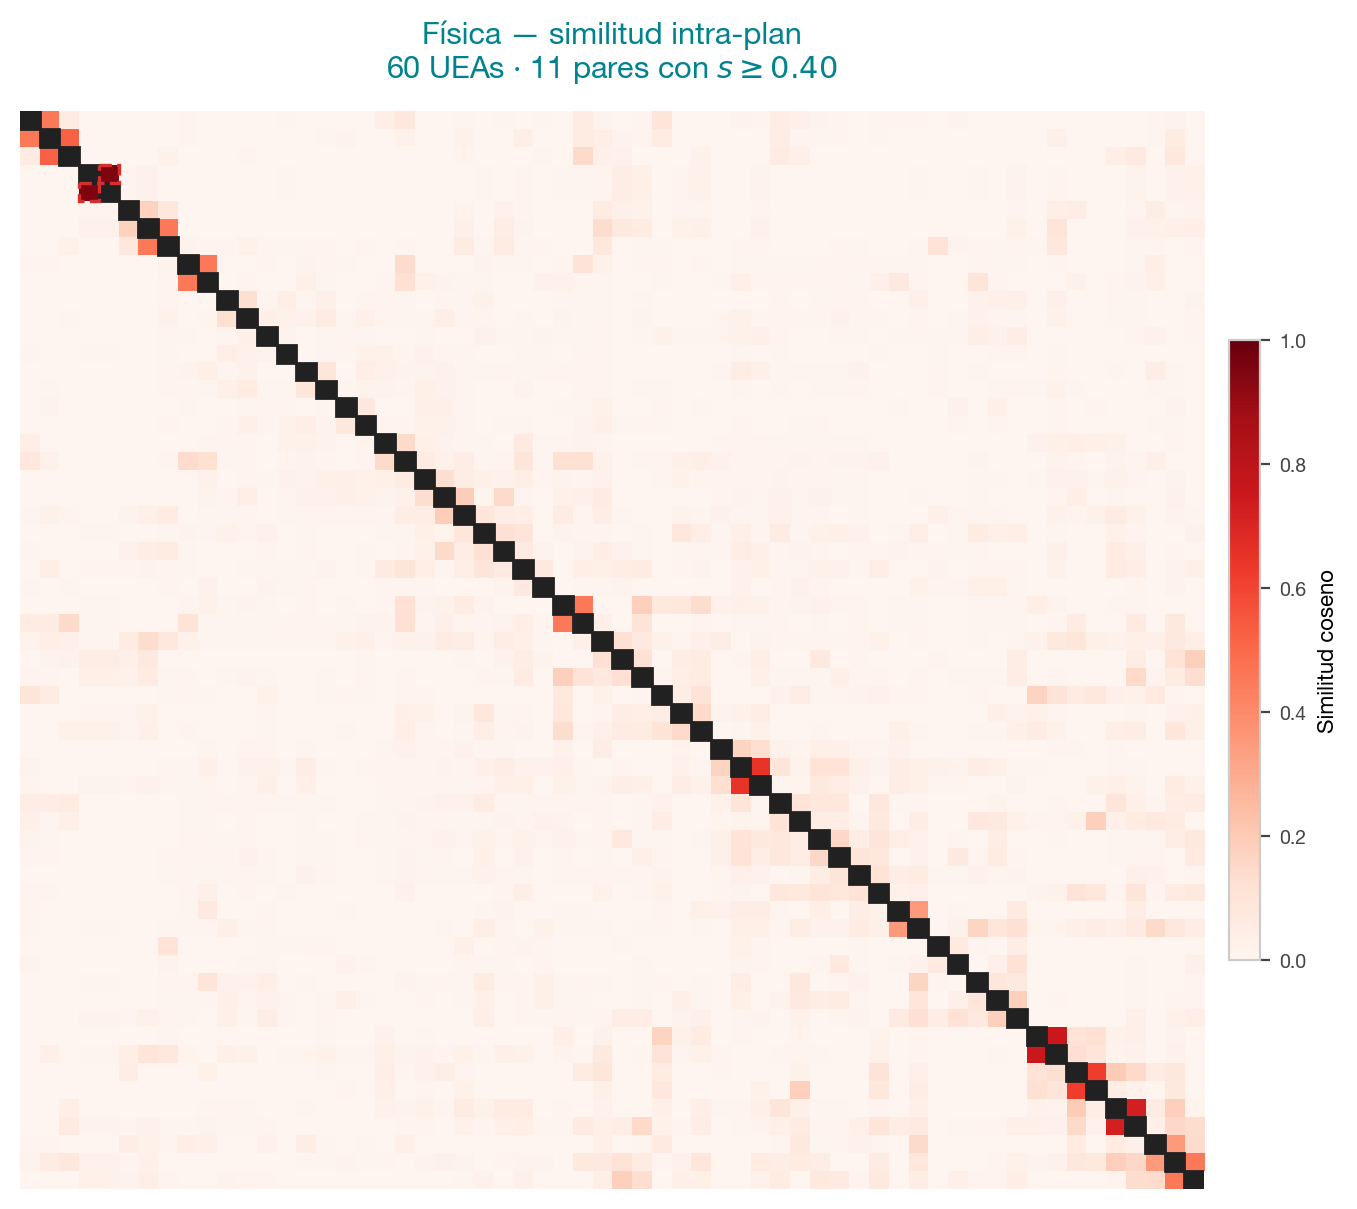
\includegraphics[width=\textwidth]{Figuras/intraplan_Fisica.png}
  \caption{Similitud intra-plan --- Física (60 UEAs, 11 pares con $s \geq 0.40$).
    El punto más brillante fuera de la diagonal es el par
    Aplicaciones Experimentales I vs.\ II ($s = 0.950$, Caso~2):
    dos UEAs consecutivas de laboratorio con programas no diferenciados.
    Los pares restantes corresponden a UEAs de cómputo científico y laboratorio.
    Ver \texttt{intraplan\_Fisica.html} para identificar UEAs individuales.}
  \label{fig:intra_fis}
\end{figure}

%%── Química ──────────────────────────────────────────────────────────────────

\paragraph{Química (55 UEAs, 11 pares con $s \geq 0.40$).}
El máximo intra-plan de Química ($s = 0.990$) es el más alto de todas las licenciaturas, correspondiente al duplicado documental de Análisis de Ciclo de Vida (Caso~1).
Los 10 pares restantes incluyen parejas teoría/laboratorio y secuencias de contenidos afines.

\begin{figure}[H]
  \centering
  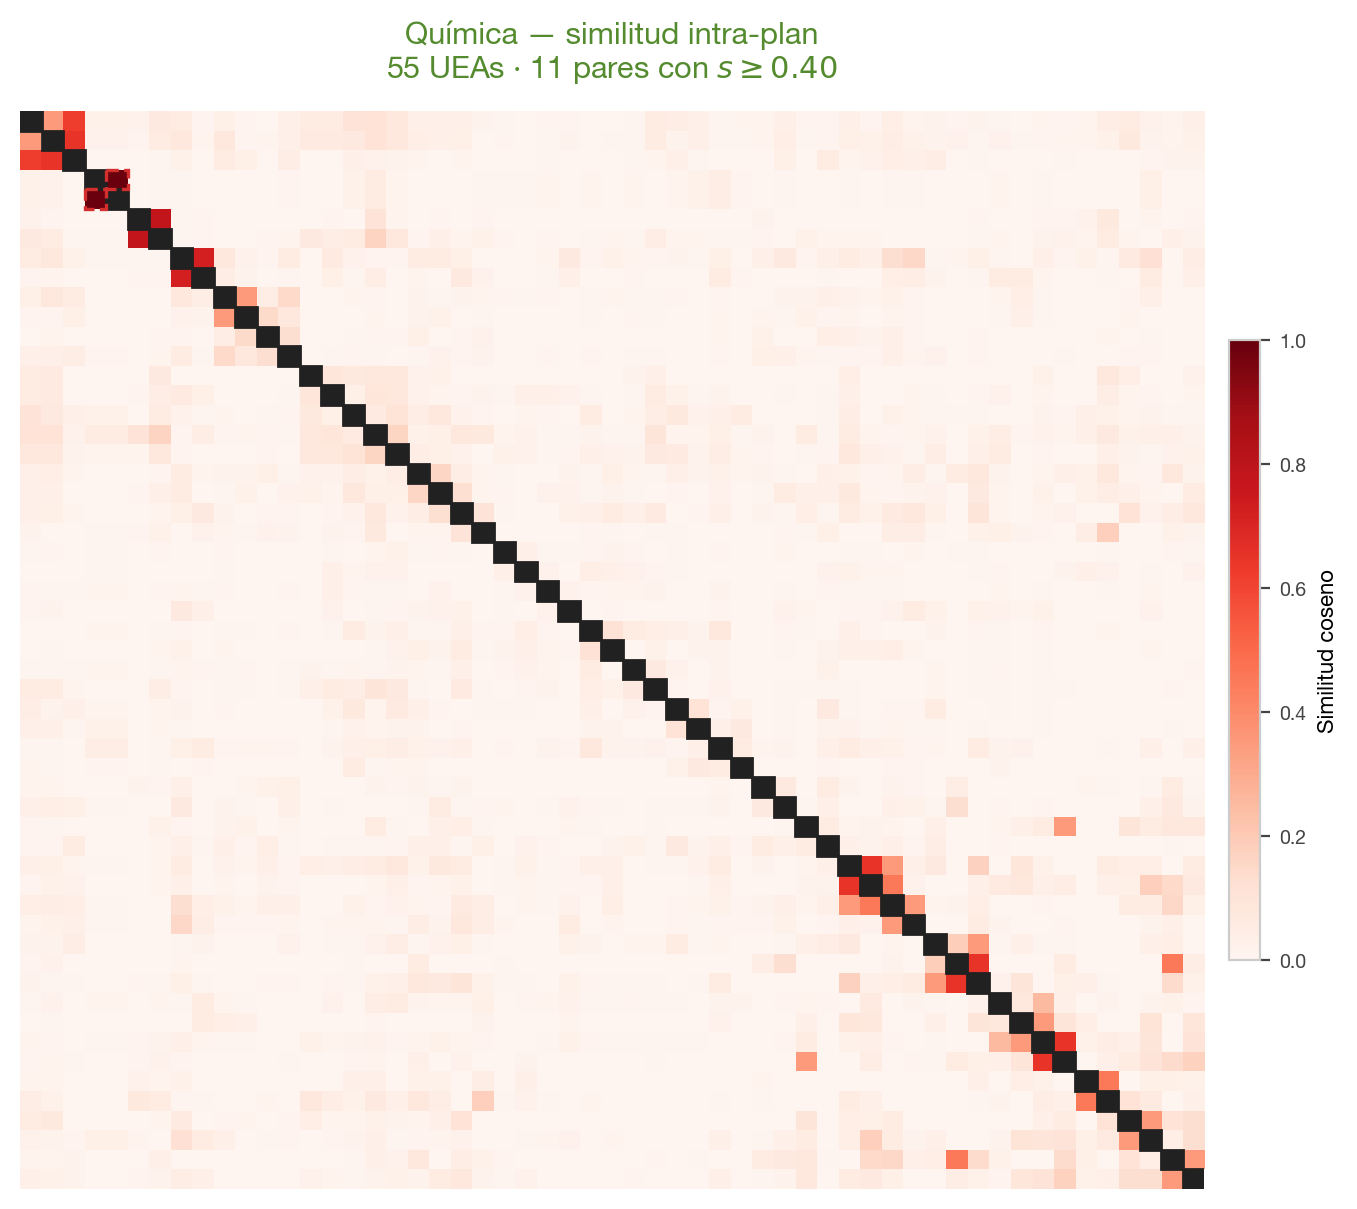
\includegraphics[width=0.76\textwidth]{Figuras/intraplan_Quimica.png}
  \caption{Similitud intra-plan --- Química (55 UEAs, 11 pares con $s \geq 0.40$).
    El punto más brillante fuera de la diagonal ($s = 0.990$) es el duplicado documental
    de \textit{Análisis de Ciclo de Vida} (Caso~1): mismo contenido en dos instancias del repositorio.
    Los demás pares son secuencias teoría/laboratorio esperadas.}
  \label{fig:intra_quim}
\end{figure}

%%── Industrial ───────────────────────────────────────────────────────────────

\paragraph{Industrial (78 UEAs, 18 pares con $s \geq 0.40$).}
Los 18 pares son en su mayoría parejas taller/teoría confirmadas: Lab.\@ de Metrología ($s = 0.85$), Lab.\@ de Conformado ($s = 0.85$), Lab.\@ de Eficiencia Operativa ($s = 0.85$), Lab.\@ Estructura de Materiales ($s = 0.78$).
El punto más brillante fuera de las parejas taller/teoría corresponde al duplicado de Herramientas Digitales en Ingeniería (caso adicional).

\begin{figure}[H]
  \centering
  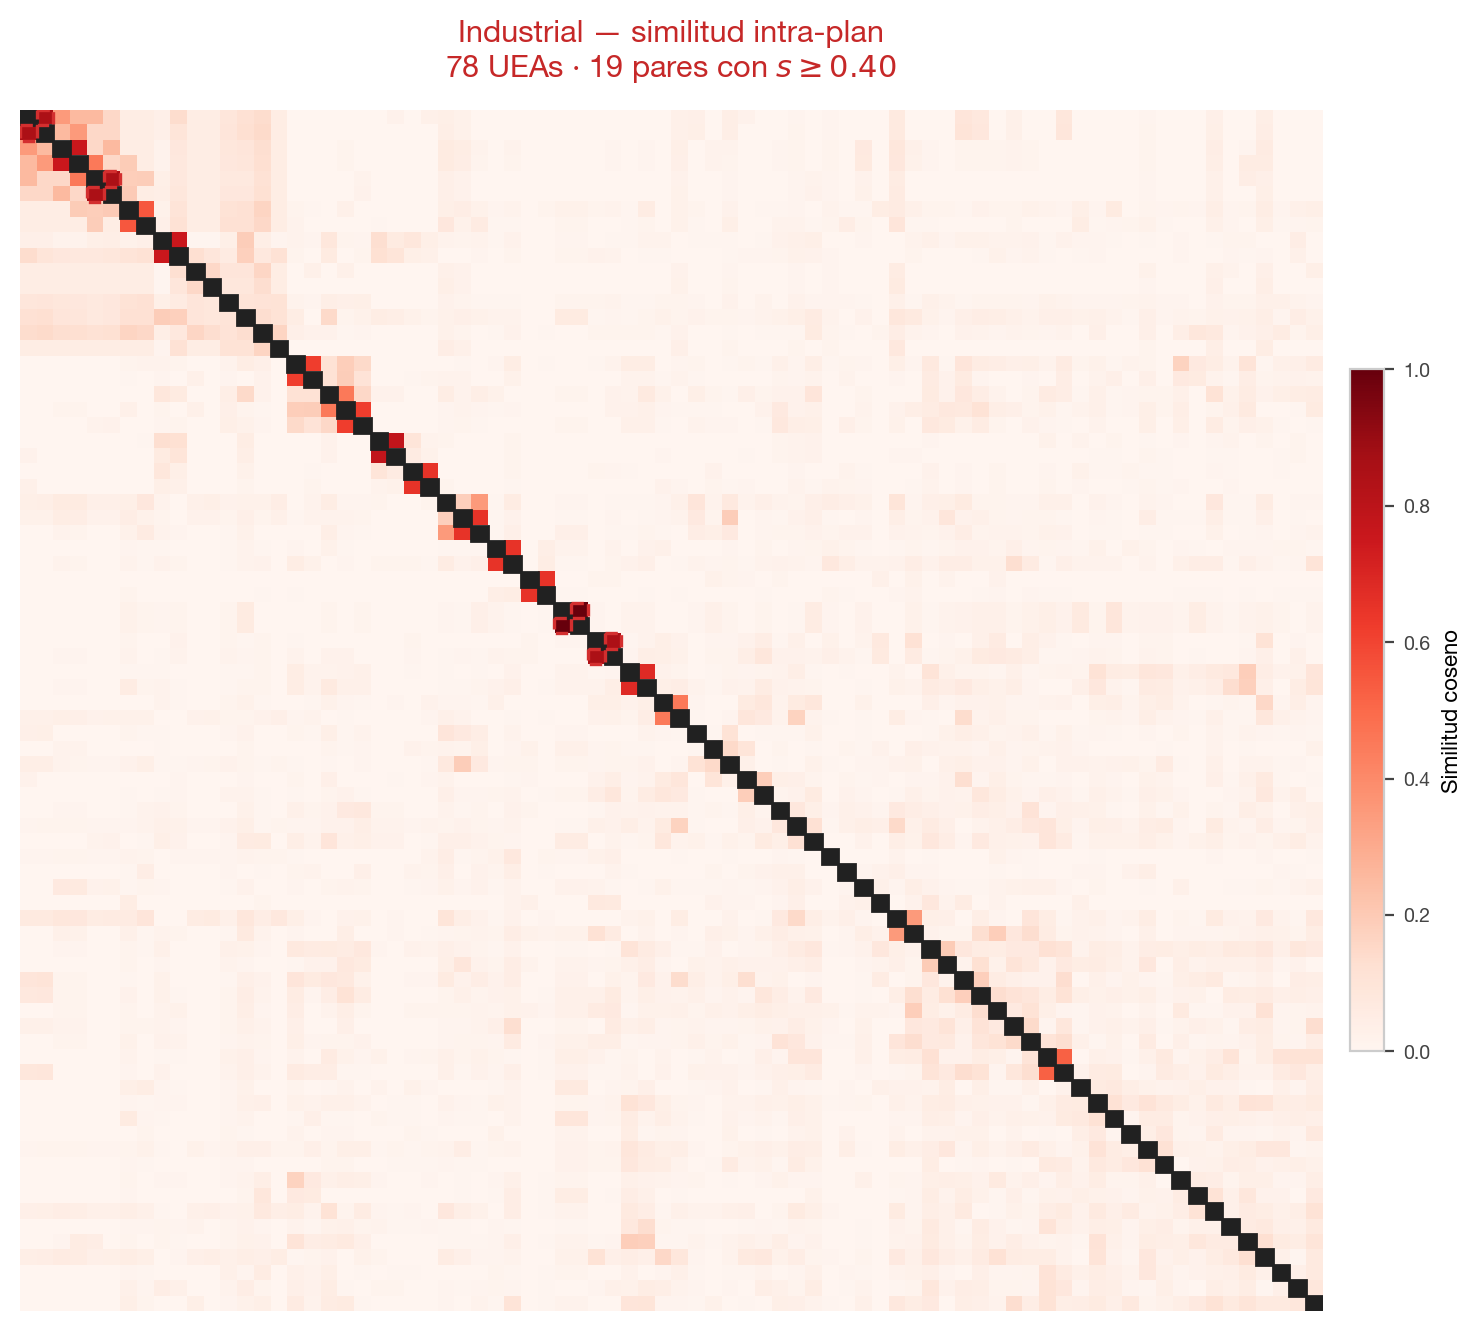
\includegraphics[width=\textwidth]{Figuras/intraplan_Industrial.png}
  \caption{Similitud intra-plan --- Industrial (78 UEAs, 18 pares con $s \geq 0.40$).
    Los bloques de la diagonal corresponden a parejas taller/teoría del área de manufactura
    (metrología, conformado, eficiencia operativa).
    El punto más brillante fuera de la diagonal es el duplicado de
    \textit{Herramientas Digitales en Ingeniería} (clave 1100202),
    identificado mediante el mapa de calor al no ser detectable por la comparación automática
    (clave idéntica).
    Ver \texttt{intraplan\_Industrial.html} para identificar UEAs individuales.}
  \label{fig:intra_ind}
\end{figure}

%%── Eléctrica ────────────────────────────────────────────────────────────────

\paragraph{Eléctrica (39 UEAs, 14 pares con $s \geq 0.40$).}
El LLM redujo los pares de 27 (TF-IDF) a 14, descartando pares atribuibles al vocabulario electromagnético compartido por Circuitos, Teoría Electromagnética y Cálculo Vectorial.
El par más significativo es Estructura de Materiales/Laboratorio de Estructura y Electroquímica ($s = 0.75$, pareja taller/teoría confirmada).

\begin{figure}[H]
  \centering
  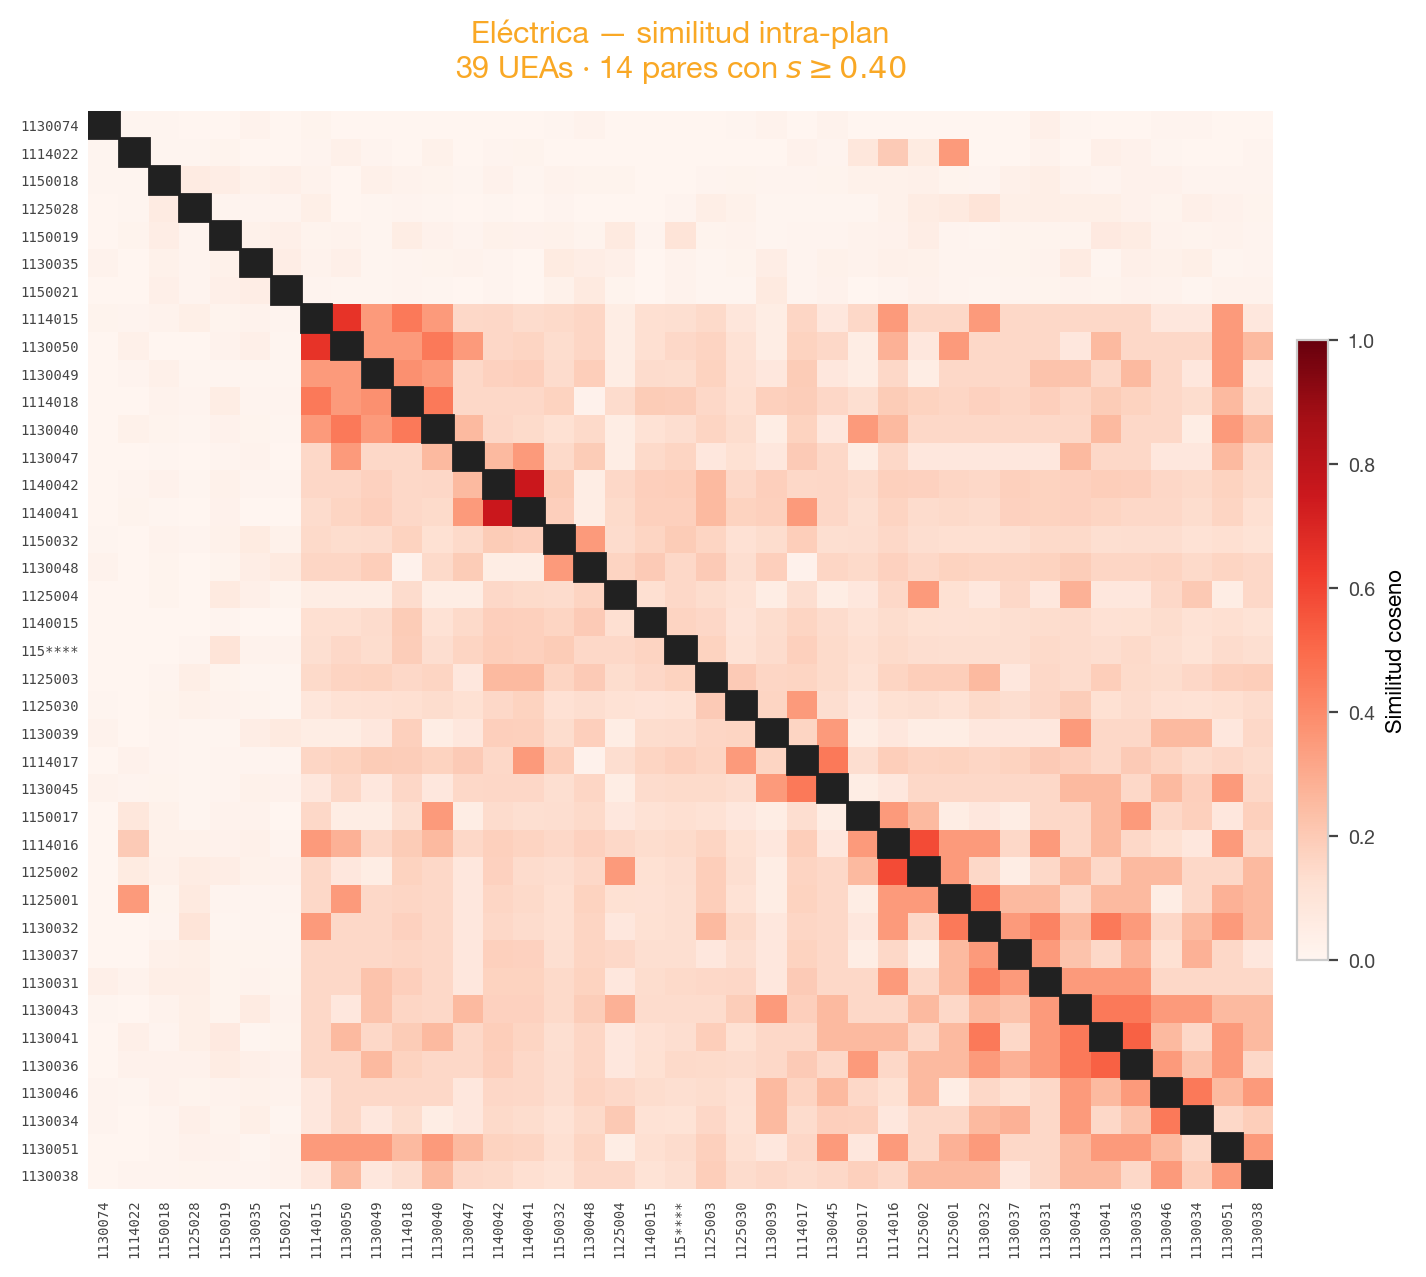
\includegraphics[width=0.76\textwidth]{Figuras/intraplan_Electrica.png}
  \caption{Similitud intra-plan --- Eléctrica (39 UEAs, 14 pares con $s \geq 0.40$).
    TF-IDF reportaba 27 pares; el LLM confirmó 14 como equivalencias reales
    y descartó 13 atribuibles al vocabulario de campo electromagnético compartido
    por Circuitos, Teoría Electromagnética y Cálculo Vectorial sin equivalencia de contenidos.}
  \label{fig:intra_elec}
\end{figure}

%%── Ambiental ────────────────────────────────────────────────────────────────

\paragraph{Ambiental (40 UEAs, 7 pares con $s \geq 0.40$).}
Traslape intra-plan bajo-moderado; los 7 pares corresponden a UEAs del área de gestión ambiental con objetivos semánticamente afines y redacciones heterogéneas.
Contrasta con el traslape inter-plan intenso con Química (14 UEAs a $s \geq 0.70$): los contenidos de Ambiental están bien diferenciados internamente, pero se solapan significativamente con los de Química.

\begin{figure}[H]
  \centering
  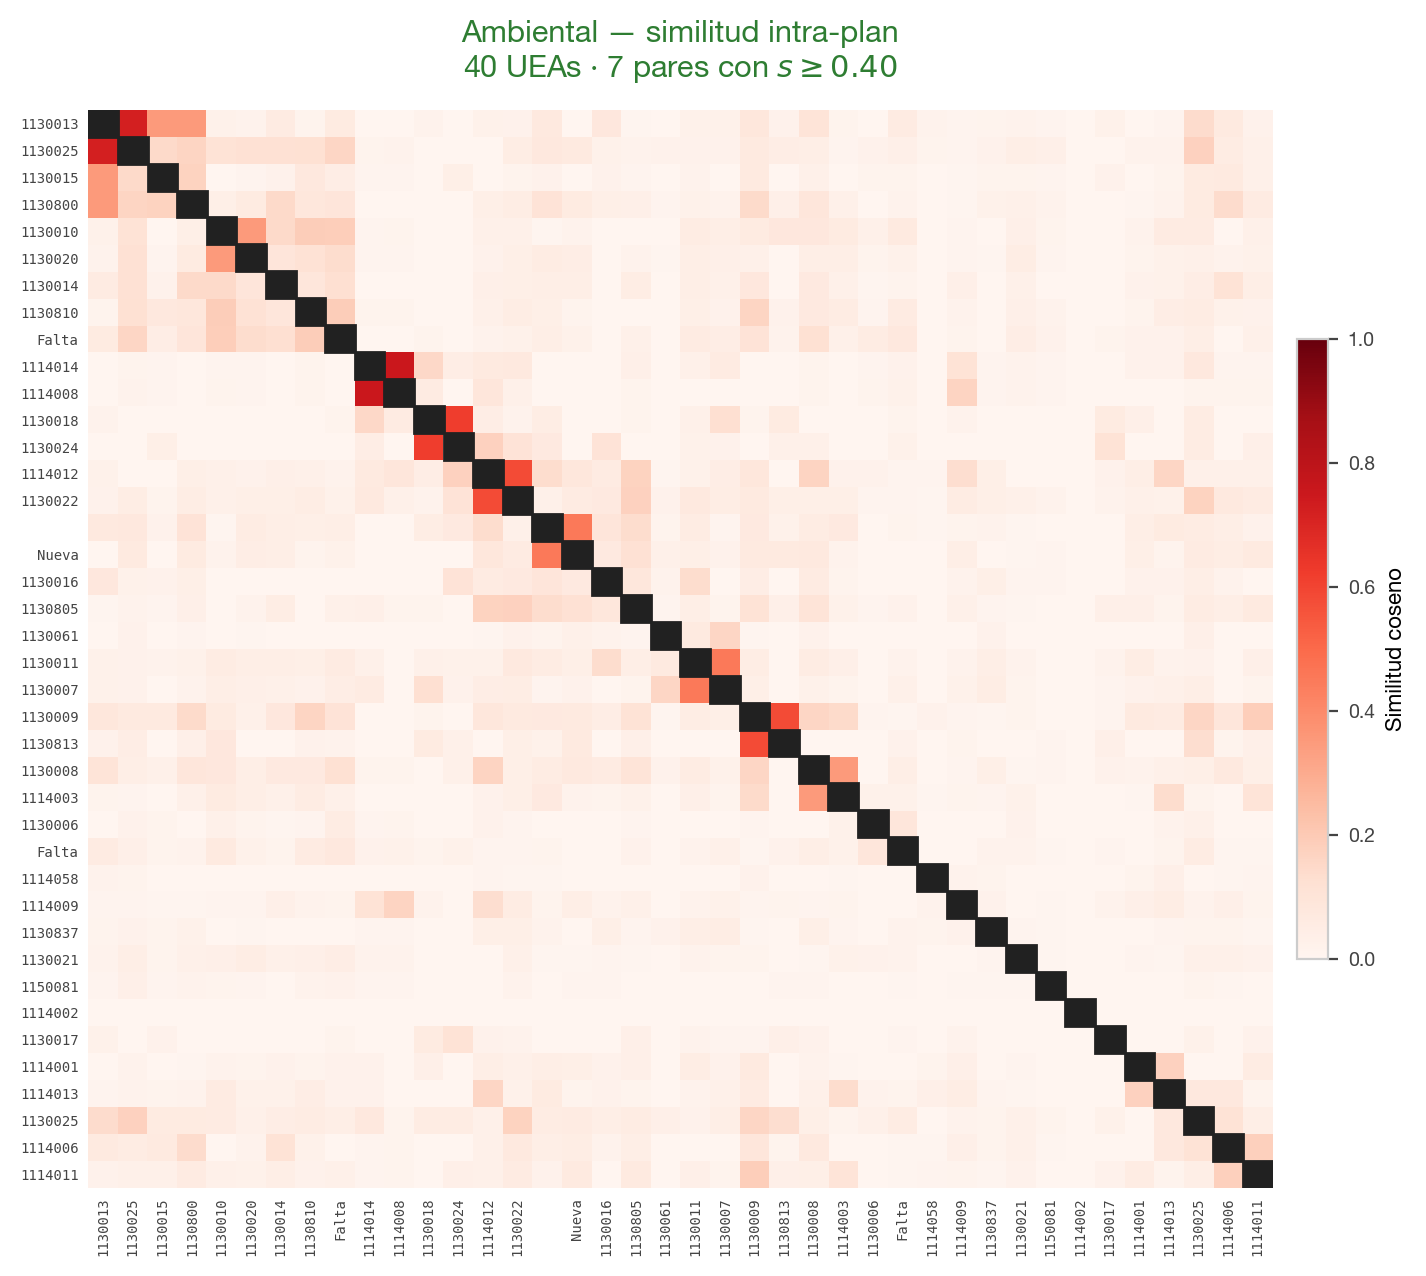
\includegraphics[width=0.76\textwidth]{Figuras/intraplan_Ambiental.png}
  \caption{Similitud intra-plan --- Ambiental (40 UEAs, 7 pares con $s \geq 0.40$, máx.\ $s = 0.750$).
    El mapa es predominantemente de color frío: plan compacto con contenidos diferenciados internamente.
    Los 7 pares son UEAs del área de gestión ambiental con objetivos afines.
    \emph{Contraste}: el traslape significativo de Ambiental es inter-plan, hacia Química
    (14 UEAs a $s \geq 0.70$, sección~\ref{sec:interplan}).}
  \label{fig:intra_amb}
\end{figure}

%%── Electrónica ──────────────────────────────────────────────────────────────

\paragraph{Electrónica (56 UEAs, 8 pares con $s \geq 0.40$).}
Electrónica tiene la menor densidad de traslape intra-plan del corpus, con 8 pares (máximo $s = 0.650$).
Sus contenidos están bien diferenciados internamente.
Sin embargo, su traslape inter-plan es intenso: 89 pares con otras licenciaturas, incluyendo pares con $s = 1.00$.

\begin{figure}[H]
  \centering
  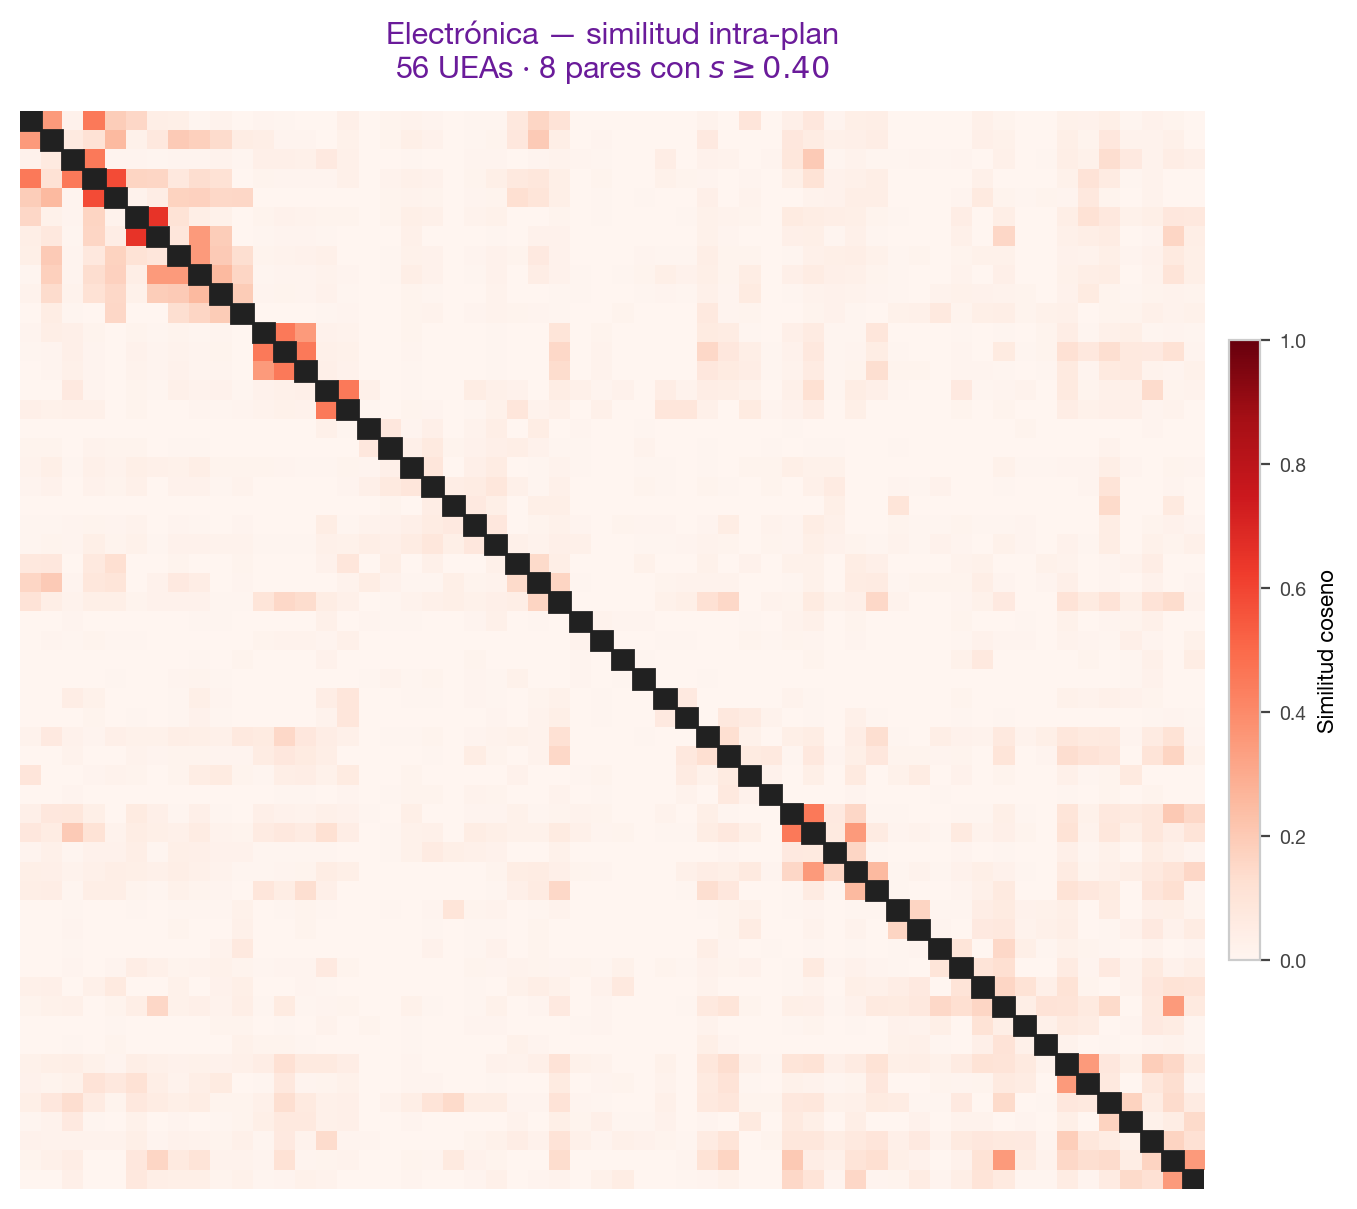
\includegraphics[width=\textwidth]{Figuras/intraplan_Electronica.png}
  \caption{Similitud intra-plan --- Electrónica (56 UEAs, 8 pares con $s \geq 0.40$, máx.\ $s = 0.650$).
    El mapa es casi completamente de color frío: plan bien diferenciado internamente.
    \emph{Contraste}: Electrónica es uno de los planes con mayor traslape \emph{inter-plan}
    (89 pares con otras licenciaturas, incluyendo $s = 1.00$)---sus UEAs son distintas
    entre sí pero equivalentes a UEAs de otros planes.
    Ver \texttt{intraplan\_Electronica.html} para identificar UEAs individuales.}
  \label{fig:intra_elecn}
\end{figure}

%% ════════════════════════════════════════════════════════════════════════════
\section{Mapa de calor agrupado}
%% ════════════════════════════════════════════════════════════════════════════

\begin{figure}[H]
  \centering
  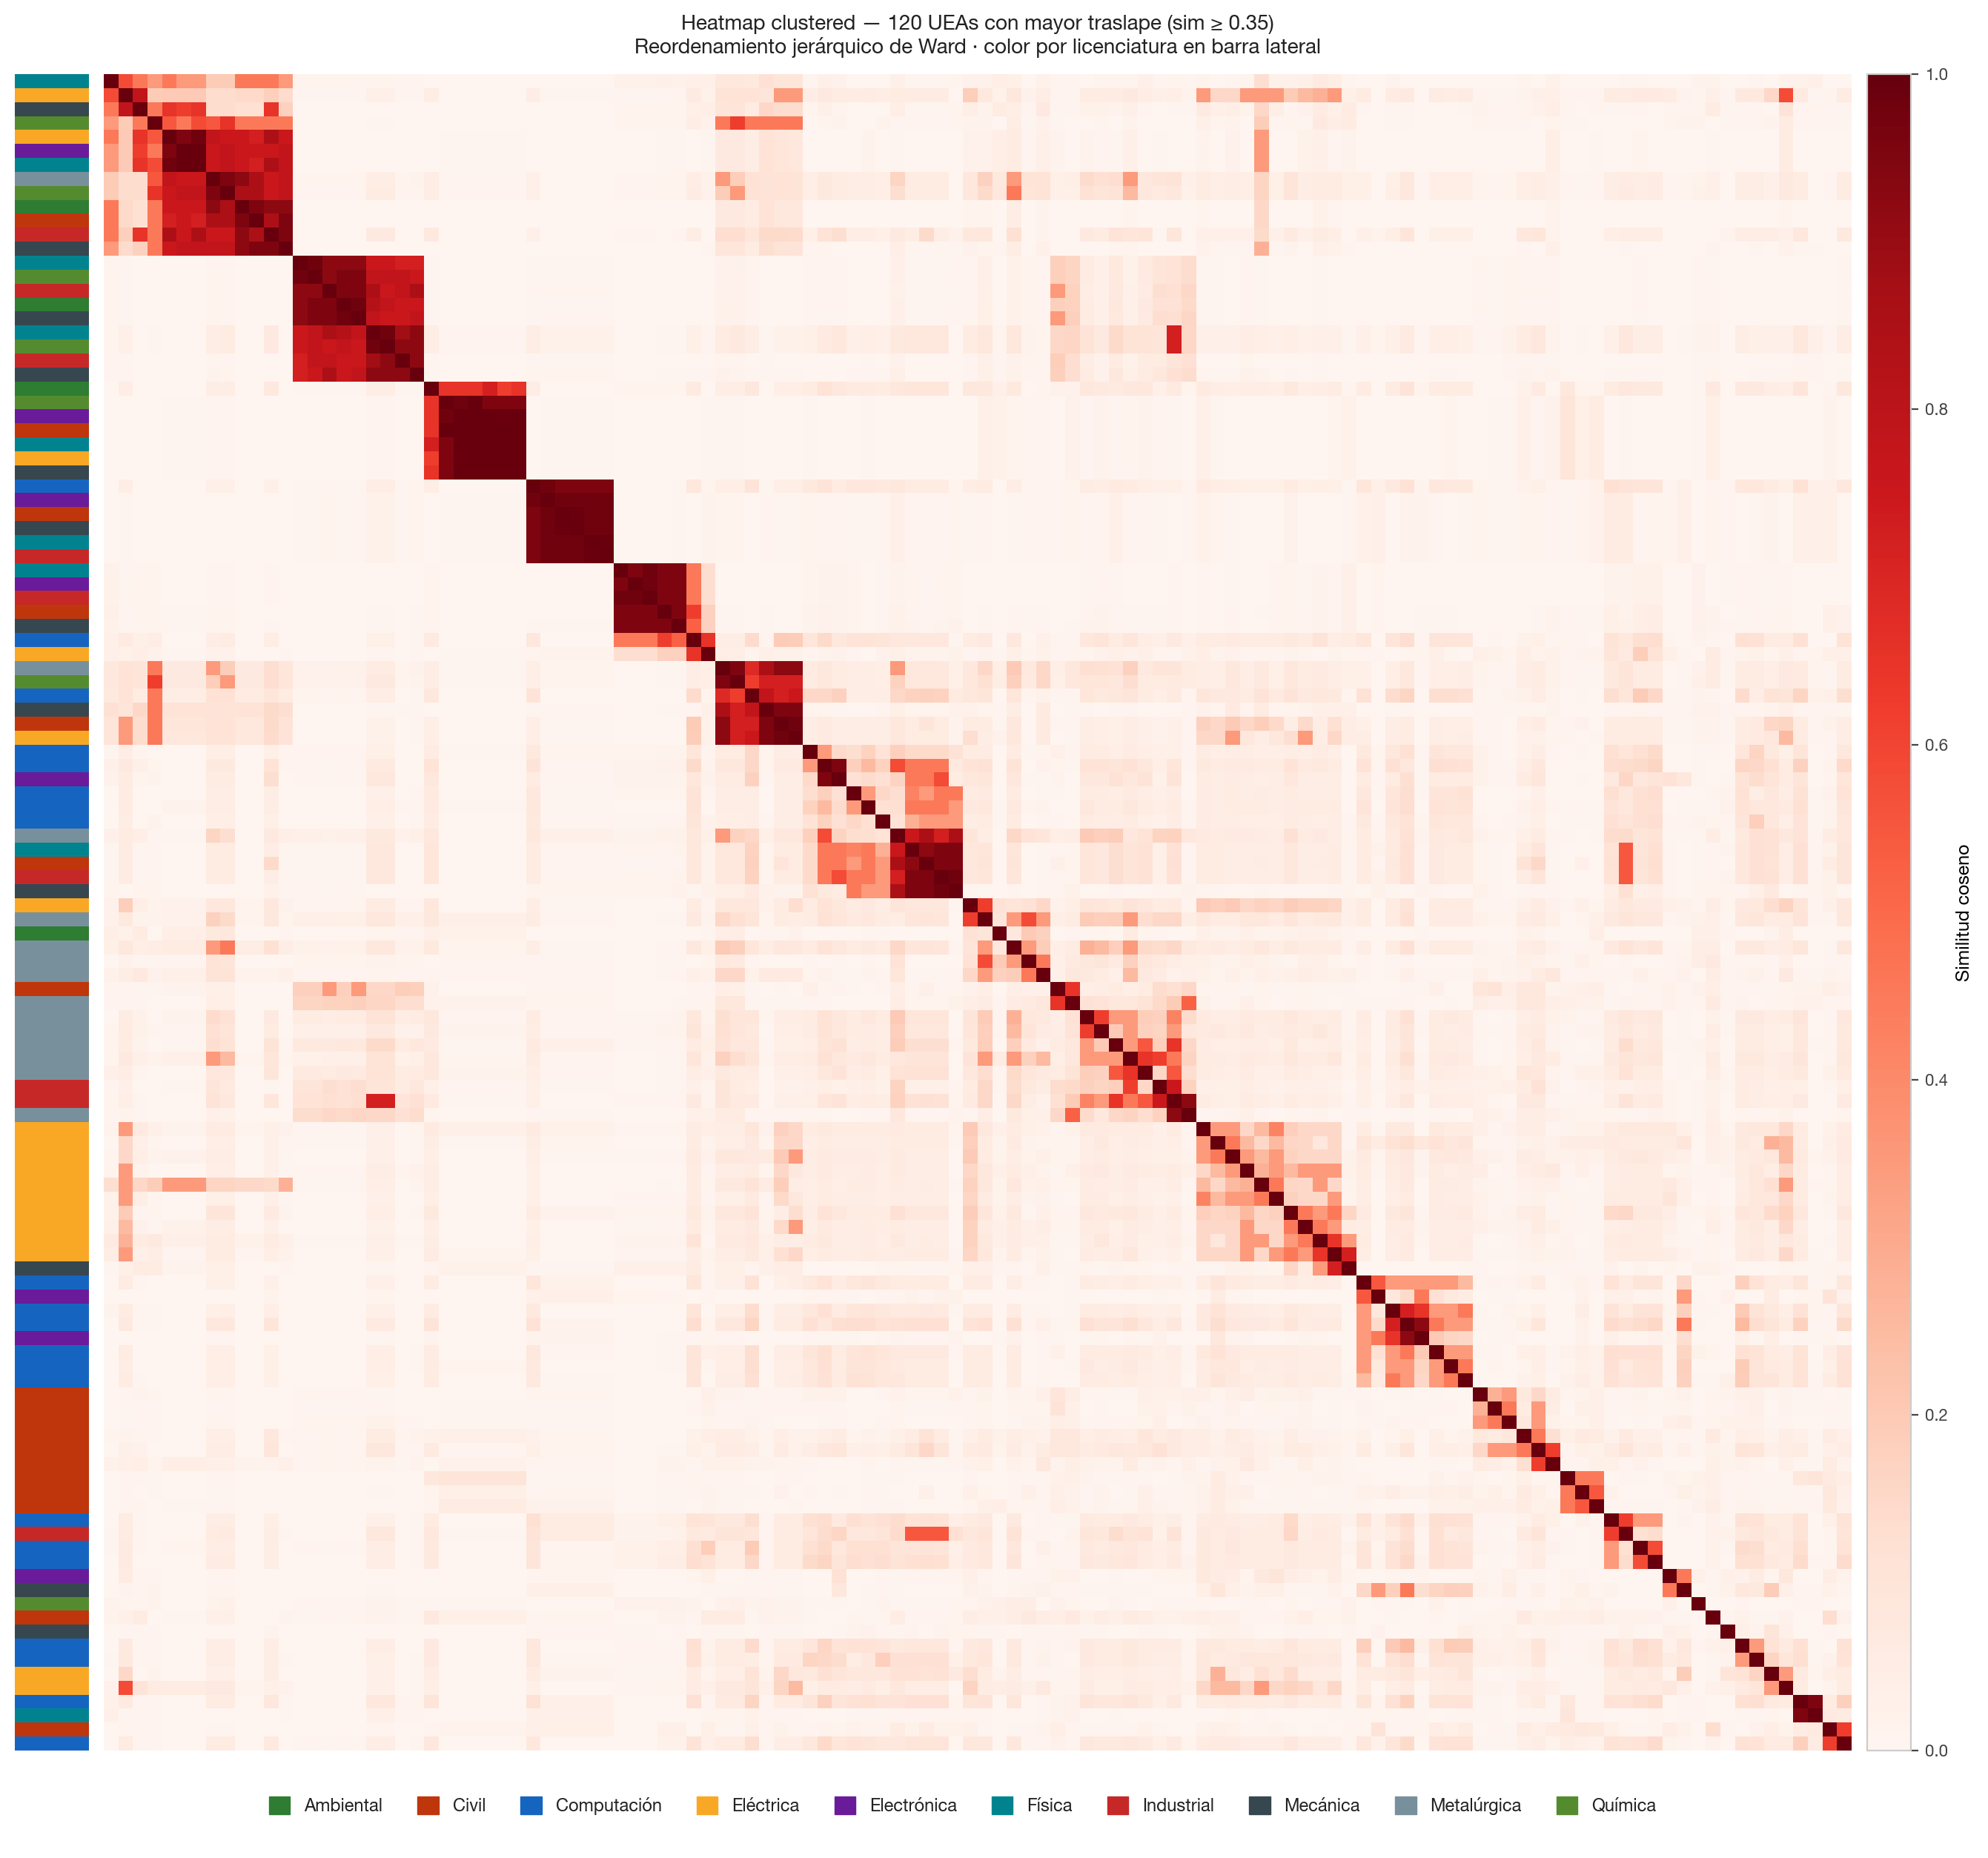
\includegraphics[width=\textwidth]{Figuras/heatmap_clustered.png}
  \caption{Mapa de calor agrupado: submatriz de similitud coseno para las 120 UEAs
    con mayor conectividad ($s \geq 0.35$), reordenadas por agrupamiento jerárquico de Ward.
    \emph{Cómo leer la figura.}
    \emph{Barra lateral izquierda}: codifica la licenciatura de cada UEA por color.
    \emph{Bloques rojos/naranja en la diagonal}: comunidades de contenido---grupos de UEAs
    que comparten vocabulario técnico.
    Si dentro de un bloque la barra lateral muestra múltiples colores,
    el traslape es inter-plan.
    \emph{Rectángulos brillantes fuera de la diagonal}: traslape bilateral entre dos
    comunidades distintas; la intensidad es proporcional a la similitud.
    \emph{Regiones frías} (amarillo pálido/blanco): independencia de contenido.
    El bloque más rojo del mapa corresponde a la comunidad Ambiental--Química.
    Ver \texttt{heatmap\_clustered.html} para identificar UEAs individuales.}
  \label{fig:clustered}
\end{figure}

Del mapa agrupado se distinguen tres comunidades de contenido.

\textbf{Comunidad~I: ingeniería ambiental compartida.}
El bloque más compacto e intenso del mapa, con barras de dos colores (Ambiental y Química), confirma el traslape bilateral documentado en la tabla~\ref{tab:matriz_interplan}.

\textbf{Comunidad~II: fenómenos de transporte y ciencia de materiales.}
Agrupa UEAs de transferencia de calor, transferencia de masa, mecánica de fluidos y termodinámica de los planes de Mecánica, Química, Ambiental e Industrial.
La diversidad de colores en la barra lateral evidencia el traslape inter-plan dentro de esta comunidad.

\textbf{Comunidad~III: matemáticas e ingeniería eléctrica/electrónica.}
Agrupa ecuaciones diferenciales, métodos numéricos y UEAs de circuitos de los planes de Eléctrica, Electrónica y Física.
Corresponde al núcleo matemático transversal de la tabla~\ref{tab:transversal}.

%% ════════════════════════════════════════════════════════════════════════════
\section{Proyección t-SNE}
%% ════════════════════════════════════════════════════════════════════════════

\begin{figure}[H]
  \centering
  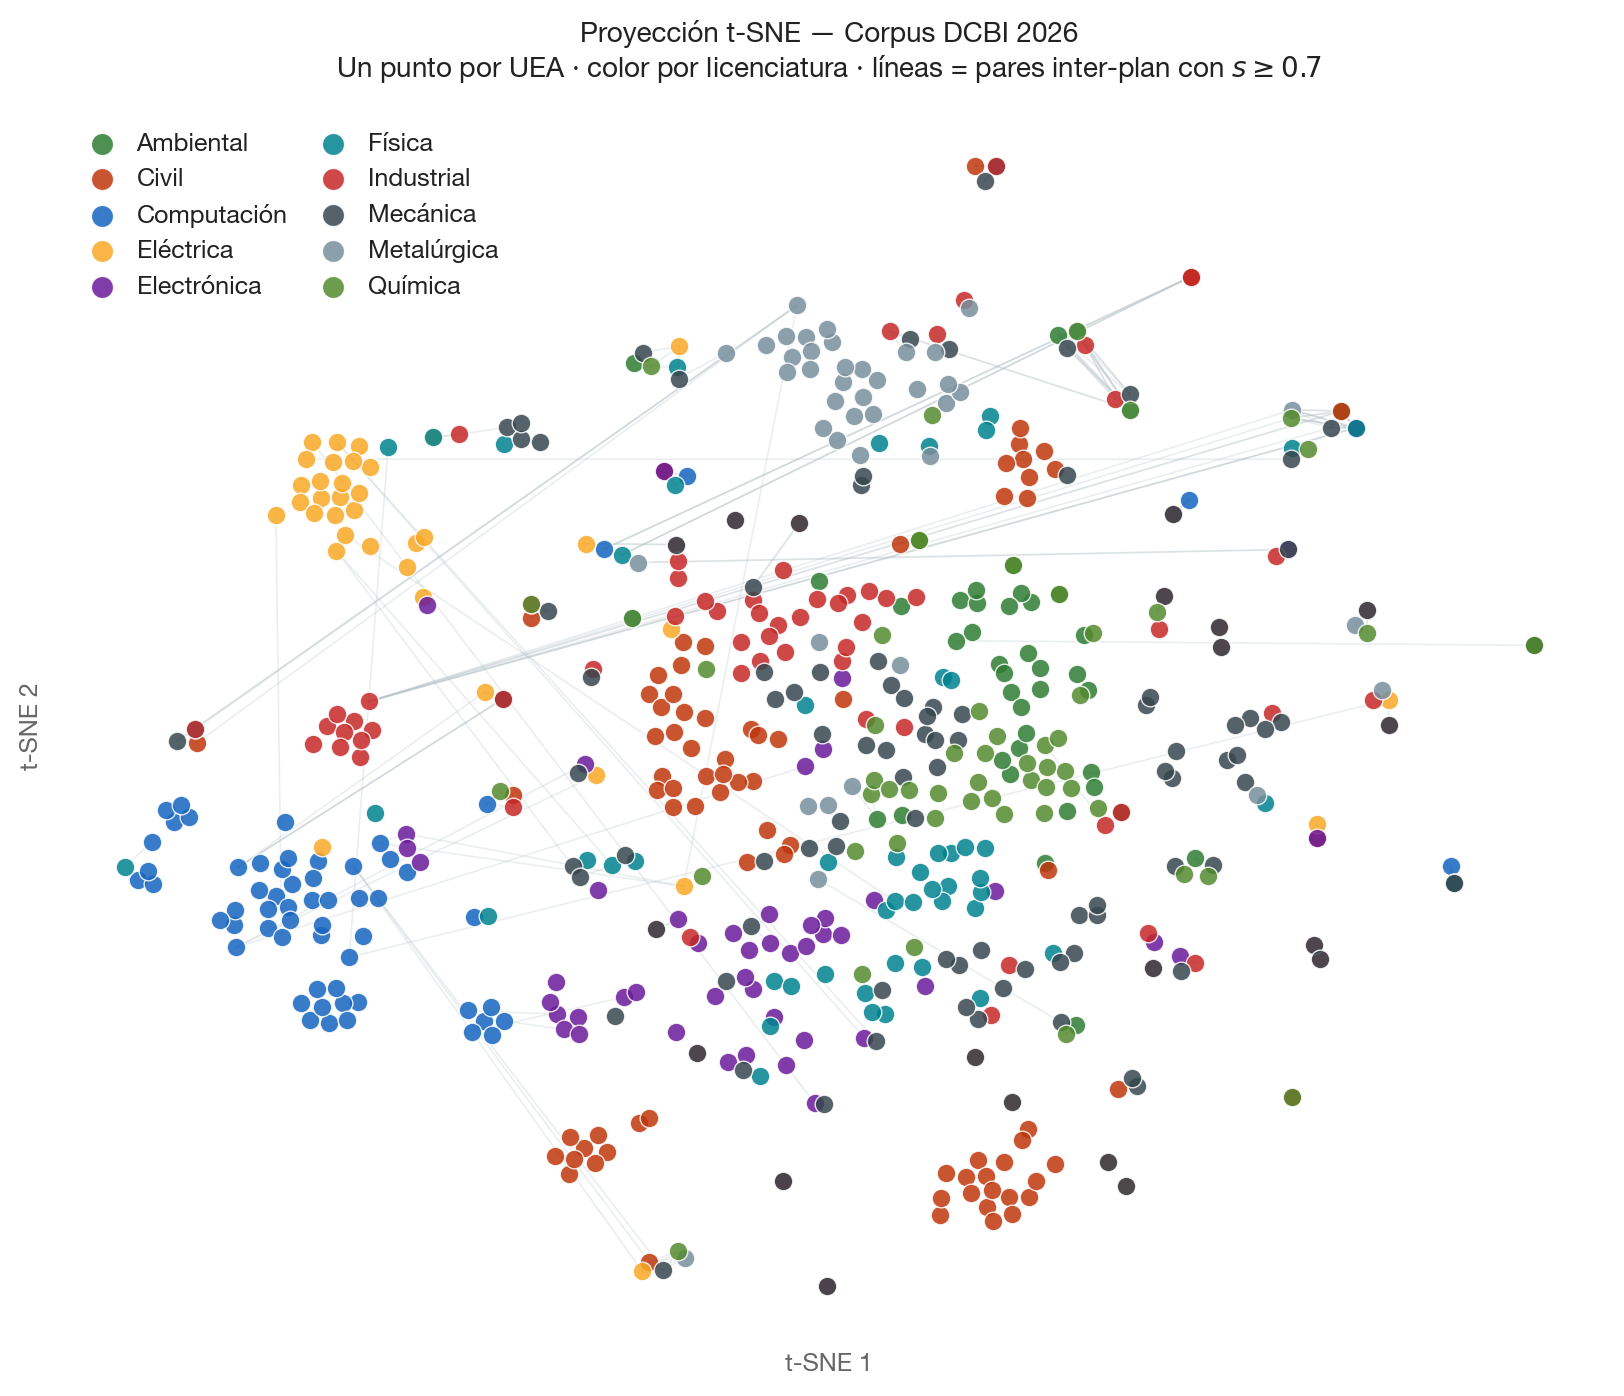
\includegraphics[width=0.88\textwidth]{Figuras/scatter_tsne.png}
  \caption{Proyección t-SNE del corpus completo (626 UEAs).
    \emph{Cómo leer la figura.}
    Cada \emph{punto} es una UEA, coloreado por licenciatura.
    \emph{Proximidad}: dos puntos cercanos comparten vocabulario técnico,
    independientemente de la licenciatura de origen.
    Un punto de color $X$ rodeado de puntos de color $Y$ indica una UEA de $X$
    con contenido similar al de varias UEAs de $Y$.
    \emph{Líneas grises}: conectan pares inter-plan con $s \geq 0.70$.
    Su brevedad confirma que t-SNE coloca las UEAs equivalentes como vecinas inmediatas
    en el plano.
    \emph{Clusters}: los grupos compactos corresponden a las comunidades disciplinares
    (ambiental/química, materiales, matemáticas/eléctrica/electrónica).
    \emph{Advertencia}: la distancia entre clusters alejados \emph{no es interpretable}---t-SNE
    preserva vecindades locales, no distancias globales.
    Ver \texttt{scatter\_tsne.html} para identificar UEAs individuales.}
  \label{fig:tsne}
\end{figure}

Los clusters visibles en la figura~\ref{fig:tsne} son coherentes con las comunidades identificadas en el mapa de calor agrupado: un grupo denso en la zona de Ambiental/Química, un bloque de UEAs matemáticas con puntos de múltiples licenciaturas superpuestos, y una región de Electrónica/Eléctrica/Física.
Las líneas grises cortas confirman que las UEAs con $s \geq 0.70$ son vecinas en el espacio de contenidos.

%% ════════════════════════════════════════════════════════════════════════════
\section{Hallazgos principales}
\label{sec:hallazgos}
%% ════════════════════════════════════════════════════════════════════════════

\subsection{Hallazgos inter-plan}

\begin{hallazgo}
\textbf{H1. Industrial--Mecánica: par de máxima densidad de traslape.}
38 UEAs compartidas a $s \geq 0.70$; 34 a $s \geq 0.85$.
Ningún otro par supera 16 UEAs a $s \geq 0.70$.
El traslape cubre manufactura, materiales, termodinámica, diseño de elementos, métodos numéricos, gestión de operaciones y UEAs de formación amplia (ética, liderazgo, comunicación).
La magnitud sugiere que ambos planes comparten implícitamente al menos un tercio de sus UEAs no-TG.
\end{hallazgo}

\begin{hallazgo}
\textbf{H2. Física: nodo de máxima conectividad transversal.}
Física comparte UEAs con todas las demás licenciaturas sin excepción: 15 con Mecánica, 14 con Industrial, 10 con Electrónica, 9 con Civil y Química, 8 con Computación, 7 con Eléctrica, 5 con Ambiental, 4 con Metalúrgica.
Con 100 pares inter-plan a $s \geq 0.30$, encabeza el corpus en conectividad transversal.
\end{hallazgo}

\begin{hallazgo}
\textbf{H3. Bloque de ingenierías clásicas.}
Mecánica, Industrial, Física y Electrónica forman un bloque con $\geq 10$ UEAs compartidas entre cada par a $s \geq 0.70$.
Civil se acopla fuertemente a Mecánica (16 UEAs) y se sitúa en la periferia de este bloque.
La densidad del bloque explica la mayor parte del traslape inter-plan del corpus.
\end{hallazgo}

\begin{hallazgo}
\textbf{H4. Ambiental--Química: núcleo de ingeniería ambiental implícito.}
14 UEAs compartidas a $s \geq 0.70$ (segunda densidad más alta del corpus, tras Industrial--Mecánica), con 9 a $s \geq 0.85$.
El conjunto incluye Análisis de Ciclo de Vida, Legislación y Gestión Ambiental, Manejo de Residuos, Procesos Biológicos, Microbiología Aplicada, Mecánica de Fluidos, Estructura y Propiedades de Materiales, entre otros.
El grado de coincidencia supera lo atribuible a vocabulario disciplinar compartido.
\end{hallazgo}

\begin{hallazgo}
\textbf{H5. Ecuaciones Diferenciales: Tronco General implícito léxico (9 de 10 planes).}
La familia de UEAs de Ecuaciones Diferenciales (Ordinarias) aparece en 9 licenciaturas con $s \geq 0.70$, bajo distintas claves en cada plan.
No fue excluida como Tronco General porque el criterio de exclusión opera por clave.
Funciona como una UEA transversal de facto: su contenido es prácticamente idéntico en nueve planes sin que exista coordinación explícita entre ellos.
\end{hallazgo}

\begin{hallazgo}
\textbf{H6. Liderazgo y Emprendimiento: Tronco General implícito semántico (9 de 10 planes).}
Contenido prácticamente idéntico en 9 licenciaturas, confirmado por el LLM ($s_{\mathrm{LLM}} \geq 0.72$).
TF-IDF le asignaba $s_{\mathrm{TF}} \approx 0.21$--$0.25$ porque su vocabulario---liderazgo, comunicación, trabajo en equipo, innovación---es genérico y filtra como baja discriminación.
Es el ejemplo más claro de equivalencia curricular estructuralmente indetectable por análisis léxico.
\end{hallazgo}

\begin{hallazgo}
\textbf{H7. Educación Ambiental y Cambio Climático: programa idéntico en 6 o más planes.}
Presente con $s \geq 0.95$ en Civil, Eléctrica, Electrónica, Física, Mecánica y Química.
La presencia en Ambiental, Industrial y Metalúrgica no ha sido verificada.
Señal de que existe un contenido transversal no coordinado entre planes.
\end{hallazgo}

\begin{hallazgo}
\textbf{H8. Núcleo matemático transversal (5 planes cada uno).}
Cálculo Integral, Probabilidad y Estadística Descriptiva, Métodos Numéricos en Ingeniería y Programación Aplicada a la Ingeniería aparecen en 5 licenciaturas con $s \geq 0.98$.
Junto con Ecuaciones Diferenciales (H5), conforman cinco UEAs matemáticas que cruzan la mayoría de los planes sin estar formalmente en el Tronco General.
\end{hallazgo}

\begin{hallazgo}
\textbf{H9. Computación--Metalúrgica: única combinación sin traslape.}
El único par de los 45 posibles con cero UEAs equivalentes a $s \geq 0.70$.
Máxima distancia curricular del corpus: los contenidos de ambas licenciaturas son ortogonales en el espacio de contenidos declarados.
\end{hallazgo}

\subsection{Hallazgos intra-plan}

\begin{hallazgo}
\textbf{H10. Duplicados documentales identificados.}
Tres casos de documentos duplicados detectados por la matriz híbrida:
\begin{itemize}[nosep,leftmargin=1.5em]
  \item \textit{Química}: Análisis de Ciclo de Vida, $s = 0.990$
    (mismo contenido, dos instancias en el repositorio).
  \item \textit{Física}: Aplicaciones Experimentales I y II, $s = 0.950$
    (programas no diferenciados entre niveles consecutivos).
  \item \textit{Industrial}: Herramientas Digitales en Ingeniería, clave 1100202 duplicada
    (identificado por mapa de calor intra-plan; no detectable por comparación automática).
\end{itemize}
\end{hallazgo}

\begin{hallazgo}
\textbf{H11. Civil: mayor densidad intra-plan (61 pares, $s \geq 0.40$).}
TF-IDF reportaba 8 pares; el LLM detectó 61.
Las áreas de estructuras, hidráulica, geotecnia y materiales del plan de Ingeniería Civil contienen objetivos convergentes redactados independientemente por departamentos distintos.
\end{hallazgo}

\begin{hallazgo}
\textbf{H12. Computación: corrección de 24 falsos positivos.}
TF-IDF reportaba 57 pares intra-plan; el LLM confirmó 33.
Los 24 pares descartados eran artefactos del vocabulario genérico de desarrollo de software.
Los 33 confirmados incluyen POO I vs.\ II y clusters de redes y bases de datos con diferenciación pedagógica insuficiente.
\end{hallazgo}

\begin{hallazgo}
\textbf{H13. Metalúrgica: mayor incremento relativo (3 → 29 pares).}
El vocabulario técnico heterogéneo entre versiones del mismo programa impedía la detección léxica.
El LLM reconoció la equivalencia semántica en 26 pares adicionales, todos parejas taller/teoría o áreas afines; no se identifican casos problemáticos.
\end{hallazgo}

\begin{hallazgo}
\textbf{H14. Impacto del enriquecimiento semántico LLM.}
Sobre 1\,505 pares candidatos a un costo de \$0.24\,USD:
\begin{itemize}[nosep,leftmargin=1.5em]
  \item 455 pares nuevos con $s_{\mathrm{LLM}} \geq 0.40$ que TF-IDF habría omitido ($s_{\mathrm{TF}} < 0.40$).
  \item Pares inter-plan detectados ($s \geq 0.30$): 154 → 391 (+154\,\%).
  \item Pares intra-plan detectados ($s \geq 0.40$): 124 → 217 (+75\,\%).
\end{itemize}
\end{hallazgo}

%% ════════════════════════════════════════════════════════════════════════════
\section{Observaciones y recomendaciones}
%% ════════════════════════════════════════════════════════════════════════════

De los hallazgos de la sección~\ref{sec:hallazgos} se desprenden cinco líneas de acción para las coordinaciones de licenciatura y las instancias de revisión curricular de la División.

\textbf{1. Corrección de duplicados documentales (H10).}
Los tres casos identificados---Análisis de Ciclo de Vida en Química, Aplic.\@ Experimentales I/II en Física, y Herramientas Digitales en Industrial---requieren revisión documental inmediata: determinar cuál es el programa vigente y retirar el duplicado del repositorio.

\textbf{2. Verificación del alcance de ``Educación Ambiental y Cambio Climático'' (H7).}
La UEA aparece con $s \geq 0.95$ en seis licenciaturas; debe verificarse su presencia en Ambiental, Industrial y Metalúrgica.
Si se confirma, el hallazgo debe elevarse a las instancias de revisión curricular para determinar el tratamiento institucional correspondiente.

\textbf{3. Documentar el traslape transversal de Ecuaciones Diferenciales y Liderazgo y Emprendimiento (H5, H6).}
Ambas UEAs tienen presencia en 9 de 10 planes con contenido prácticamente idéntico sin coordinación explícita entre licenciaturas.
El hallazgo documenta esta situación para conocimiento de las instancias de revisión curricular; cualquier decisión sobre su tratamiento corresponde al proceso académico institucional.

\textbf{4. Revisión del núcleo disciplinar Ambiental--Química y del traslape intra-plan de Civil (H4, H11).}
El bloque Ambiental--Química concentra más de 14 UEAs equivalentes a $s \geq 0.70$.
Civil registra 61 pares intra-plan, atribuibles a objetivos convergentes redactados independientemente.
En ambos casos se recomienda examinar si el traslape responde a una decisión curricular explícita o es resultado no intencional, y documentarlo a través de los mecanismos que la División considere pertinentes.

\textbf{5. Diferenciación de contenidos en Computación (H12).}
Los 33 pares intra-plan confirmados incluyen casos de diferenciación pedagógica insuficiente: POO I vs.\  II y los clusters de redes y bases de datos.
Se recomienda una revisión específica del plan de Computación para establecer diferenciación clara entre UEAs consecutivas y entre UEAs de áreas temáticas próximas.

\begin{notabox}
Las métricas de este reporte se basan exclusivamente en el texto de los campos
\textit{Objetivo General} y \textit{Contenido Sintético} de los programas de UEA tal
como están registrados en los documentos del repositorio DCBI 2026.
Una similitud baja no implica que dos UEAs no compartan bibliografía o metodologías;
una similitud alta no implica que las UEAs deban fusionarse, sino que sus contenidos
declarados requieren revisión y diferenciación explícita.
\end{notabox}

%% ════════════════════════════════════════════════════════════════════════════
\bibliographystyle{plainnat}
\bibliography{similitud_refs}
%% ════════════════════════════════════════════════════════════════════════════

\end{document}
